\documentclass[11pt, a4paper]{article}

\usepackage[utf8]{inputenc}
\usepackage{amsmath}
\usepackage{amsfonts}
\usepackage{amssymb}
\usepackage{graphicx}
\usepackage{caption}
\usepackage{subcaption}
\usepackage{enumitem}
\usepackage{secdot}
\usepackage{csquotes}
\usepackage{booktabs}
\usepackage{multirow}
\usepackage{hyperref}
\usepackage{bm}
\usepackage{framed}
\usepackage{xcolor}
\usepackage{multicol}
\usepackage[authoryear]{natbib}
\usepackage[margin=0.9in]{geometry}
\usepackage[most]{tcolorbox}
\usepackage{verbatim}
\usepackage{soul}
\usepackage[yyyymmdd]{datetime}
\usepackage{pdflscape}
\usepackage{rotating}
\usepackage{hvfloat}
\usepackage{mathtools}
\usepackage{bbm}
\usepackage{algorithm}
\usepackage{algpseudocode}

\allowdisplaybreaks

\newtcolorbox{tcbdoublebox}[1][]{%
  enhanced jigsaw,
  sharp corners,
  colback=white,
  borderline={1pt}{-2pt}{black},
  fontupper={\setlength{\parindent}{20pt}},
  #1
}

\hypersetup{
    colorlinks,
    linkcolor={red!40!black},
    citecolor={blue!40!black},
    urlcolor={blue!80!black}
}

\newcommand{\R}{{\ensuremath{\mathbb{R}}}}
\newcommand{\N}{{\ensuremath{\mathbb{N}}}}
\newcommand{\Q}{{\ensuremath{\mathbb{Q}}}}
\newcommand{\Z}{{\ensuremath{\mathbb{Z}}}}

\algnewcommand\algorithmicforeach{\textbf{for each}}
\algdef{S}[FOR]{ForEach}[1]{\algorithmicforeach\ #1\ \algorithmicdo}

\DeclareMathOperator*{\argmin}{\arg\,\min}
\DeclareMathOperator*{\argmax}{\arg\,\max}
\newcommand{\indep}{\perp \!\!\! \perp}
\newcommand{\cond}{\!~|~\!}
\setlength{\footnotesep}{0.8\baselineskip}
\setlength{\parskip}{0.7\baselineskip}
\renewcommand\arraystretch{1.2}
%\renewcommand\refname{Bibliografía}

\providecommand{\keywords}[1]{
\begin{tabular}{r p{10cm}}
\textbf{Keywords:} & #1
\end{tabular}}

% \counterwithin*{equation}{section}% Reset equation at \section
% \counterwithin*{equation}{subsection}% Reset equation at \subsection
% \renewcommand{\theequation}{\thesection.\arabic{equation}}

\title{Research Project:\\On a (more) flexible class of Latent Variable Model}
\author{Camilo Cárdenas-Hurtado}%\\Irini Moustaki \\Giampiero Marra} %\\\href{c.a.cardenas-hurtado@lse.ac.uk}{(c.a.cardenas-hurtado@lse.ac.uk)}\\London School of Economics and Political Science}
\date{This version: \longdate \today, at \currenttime}


\begin{document}

\maketitle

\begin{abstract}
The Generalized Linear Latent Variable Model (GLLVM) is a general class of statistical model commonly used in multivariate data analysis to explain the underlying relationships between observed random variables and to reduce data dimensionality. To do so, associations between $p$ observed variables are explained through a set of $q$ latent variables (factors) that belong in a lower dimensional vector space, i.e., $q \ll p$. Despite of being a powerful modelling tool, the GLLVM faces limitations when we fail to meet common modelling assumptions, such as linearity or homoscedasticity. In this paper we expand the class of GLLVMs by accommodating measurement equations on the location, scale and shape parameters of the univariate (conditional) distributions for each of the $p$ manifest variables. In our model, the semiparametric latent variable model (SPLVM), we specify measurement equations that follow a generalized additive model specification, allowing for (possibly) nonlinear relationships between manifest and latent variables in their first (mean), second (variance), and higher order moments (skewness and kurtosis).
\end{abstract}

\keywords{\hl{[Keywords go here]}}

\section{Introduction}

Many research questions in the Social and Behavioral sciences involve the analysis of multivariate data that is measured on binary, categorical (nominal or ordinal) and/or metric (discrete or continuous) scales. The analysis of mixed data aims to find hidden patterns and to simplify its complex structure. The generalized linear latent variable model (GLLVM, \citealp{BKM2011}) is a unified statistical framework that helps to achieve these goals. Either in an exploratory or a confirmatory fashion, latent variable models (LVM) are used to reduce the dimensionality of the observed variables by explaining their associations through a lower dimensional set of latent variables (factors). More formally, let $\mathbf{y} = (y_1,...,y_p)'$ be a vector of observed variables and $\mathbf{z} = (z_1,...,z_q)'$ a vector of factors, with $q \ll p$. Jointly, ($\mathbf{y}, \mathbf{z}$) corresponds to a (single) realization from a joint probability distribution that can be expressed as
\begin{equation}
 f(\mathbf{y}, \mathbf{z}) = f(\mathbf{y}\cond\mathbf{z})~p(\mathbf{z}). \label{eq:thLVM}
\end{equation}
The conditional probability function $f(\mathbf{y}\cond \mathbf{z})$ is known as the measurement component of the LVM, and describes how $\mathbf{y}$ is a `manifestation' of the set of factors $\mathbf{z}$. The probability function $p(\mathbf{z})$ is the structural part of the LVM, and specifies the joint distribution of the latent variables.

The LVM in equation \eqref{eq:thLVM} represents a very general class of statistical models that encompasses the generalized mixed/random effects model \citep{Laird&Ware_Biometrics1982, Zeger&Karim_JASA1991, Lee&Nelder_JRSS1996, Lee&Nelder_Biometrika2001, Lee&Nelder_JRSS2006}, the factor analysis model \citep{Lawley&Maxwell_JRSS1962, LM1971}, the structural equation model (LISREL, \citealp{Joreskog_Biometrika1970, Joreskog_ETS1970, Joreskog_1973}, and SEM, \citealp{Bollen1989}), and the class of item response theory models (IRT, \citealp{LN1968, Bartholomew_JRSS1980, Bock&Aitkin_Psychometrika1981, BK1999}). The main difference between these frameworks lies on the specific distributional assumptions and restrictions placed on $f(\mathbf{y} \cond \mathbf{z})$ and $p(\mathbf{z})$ to achieve interpretation, dimensionality reduction, and parameter identifiability.

%For instance, albeit the distribution of the latent variables in equation (\ref{eq:thLVM}) is, in principle, entirely arbitrary \citep{Bartholomew_Biometrika1984}, $p(\mathbf{z})$ is often assumed to be a (standard) multivariate normal distribution. For example, in factor models the parameters in the covariance matrix in $p(\mathbf{z})$ are freely estimated, in IRT models the covariances are set to zero, while in the SEM literature either an unstructured covariance matrix or a linear or non-linear model is specified for the relationships among latent and explanatory variables.

In the LVM literature an important assumption is that of \textit{local independence}. This latter states that the associations between manifest variables are assumed to be entirely explained by the latent variables, and therefore, the observed variables are independent from each other conditional on the latent factors, $f(\mathbf{y}\cond\mathbf{z}) = \prod_{i=1}^p f_i(y_i\cond\mathbf{z})$. This allows us to assume different measurement models for each manifest variable. In particular, for $i=1,...,p$, the GLLVM framework assumes that $f_i(y_i\cond\mathbf{z})$ is a distribution from the exponential family with canonical parameter $\zeta_i$ and scale parameter $\phi_i$, expressed in the form
\begin{equation}
f_i(y_i \cond \mathbf{z}; \zeta_i,\phi_i) = \exp\left\{\frac{y_i\zeta_i(\mathbf{z}) - b(\zeta_i(\mathbf{z}))}{\phi_i} + c(y_i;\phi_i)\right\}, \label{eq:expd}
\end{equation}
where the notation $\zeta_i(\mathbf{z})$ means that the canonical parameter is a function of the latent variables $\mathbf{z}$. For notational economy, let $\zeta_i(\mathbf{z}) \equiv \zeta_i$. Recall that for the two-parameter exponential family, $\mathbb{E}(y_i\cond\mathbf{z}) = \mu_i = b'(\zeta_i) = \partial b(\zeta_i)/ \partial \zeta_i$ and var$(y_i\cond\mathbf{z}) = \phi_i b''(\zeta_i) = \phi_i\partial \mu_i/ \partial \zeta_i$.

Along the lines of the generalized linear model framework (GLM, \citealp{Nelder&Wedderburn_JofRSS1972, MN1989}), the relationship between the manifest and latent variables is usually assumed to be linear through $\zeta_i$, with a systematic component or linear predictor, $\eta_i$, such that for every $i=1,...,p$,
\begin{equation}
  \zeta_i = \eta_i = \alpha_{i0} + \sum_{j=1}^q \alpha_{ij} z_j \label{eq:linLVM}
\end{equation}
where $\alpha_{i0}$ is an intercept term and the slope parameters $\alpha_{ij}$ are also known as factor loadings. For notational convenience, let $\bm{\alpha}_i = (\alpha_{i0}, \alpha_{i1},..., \alpha_{iq})'$. The linear equation \eqref{eq:linLVM} can be viewed as a particular case of the more general setting $\zeta_i = \eta_i = g_i(\mathbf{z}; \bm{\alpha}_i)$, where $g_i:\R^{q} \to \R$ is a continuous function on $\mathbf{z}$ with parameters $\bm{\alpha}_i$. For notational economy, we denote $g_i(\mathbf{z}; \bm{\alpha}_i) \equiv g_i(\mathbf{z})$. Additionally, we choose a monotonic and differentiable linking function, $\upsilon_i:\R \to \R$, such that $\eta_i = \upsilon_i(\mu_i) = (b')^{-1}(\mu_i)$, where the function $(b')^{-1}(\cdot)$ denotes the inverse mapping of the function $b'(\cdot)$. The link function relates the systematic component $\eta_i$ to the location parameter $\mu_i$ of the response variable $y_i$. This GLM-type formulation allows for modeling the (conditional) mean of the manifest variables as a (linear) function of the latent factors. However, while the conditional variance can be expressed in terms of the mean parameter (i.e., var$(y_i\cond\mathbf{z})$ is a function of $\mu_i$), other higher order moments of the manifest variables, like the kurtosis and the skewness, are usually not modeled explicitly in terms of the latent variables $\mathbf{z}$ (or any other set of covariates).

Despite its functionality, the linearity assumption in the GLLVM might not be appropriate in settings in which is reasonable to consider nonlinear relationships between manifest and latent variables. For example, in education testing, easier items might have poor discrimination power among high-ability subjects (and vice-versa), suggesting a possible nonlinear relationship between the test score and the respondents' abilities. In psychology tests, unobservable variables, such as concentration capacity, can have nonlinear effects on both attention span or response timing (measured in minutes). In economics, `consumer confidence' or `willingness to spend' can have nonlinear relationships with the expenditure on different types of goods and services.

Indeed, the structure of $g_i$ in equation \eqref{eq:linLVM} can be relaxed to accommodate nonlinear functional forms. Works on nonlinear factor analysis started with \citet{McDonald_Psychometrika1962, McDonald_BJMSP1965, McDonald_BJMSP1967, McDonald_Psychometrika1967} and \citet{Etezadi-Amoli&McDonald_Psychometrika1983}, who discussed a least squares (LS) estimation for the factor loadings in a nonlinear (but with known functional form) measurement equation. In a similar fashion, \citet{Yalcin&Amemiya_StatSci2001} presented a method of moments (MM) procedure, while \citet{Rizopoulos&Moustaki_BJMSP2008} extend the GLVM to include nonlinear (and covariate) effects under a full information ML framework. \citet{Zhu&Lee_BJMSP1999} presented a Bayesian nonlinear factor model. These authors assumed a nonlinear but known functional forms for $g_i$, usually involving lower order polynomials (e.g., quadratic forms) and interactions between latent variables. For an overview of developments and origins of the nonlinear factor analysis refer to \citet{Wall&Amemiya_FA2007}.

%Non-normal items can be either to: a) nonlinear relationships of a normal latent variable (and similar to the underlying variable approach); or b) linear relationships of a non-normal latent variable (\citep{Klein&Moosbrugger_Psychometrika2000}).

It is worth noting that nonlinear and interaction effects have been also studied in the SEM literature (see, e.g. \citealp{Kenny&Judd_PsychBull1984, Arminger&Muthen_Psychometrika1998, Klein&Moosbrugger_Psychometrika2000, Wall&Amemiya_JofEdBehSta2001, Lee&Zhu_Psychometrika2002, Bauer_SEM2005, Fahrmeir&Raach_Psychometrika2007, Yang&Dunson_Psychometrika2010,  Kelava&Nagengast_MultBehRes2012}, among others, and the references therein). These papers consider nonlinear relationships among latent variables, but, in most cases, assume a linear structure in the measurement equations. In particular settings (see, e.g., \citeauthor{Kenny&Judd_PsychBull1984}'s approach), auxiliary measurement equations involving interactions between items or squared terms, as well as nonlinear constraints on the regression coefficients, are needed for correct factor loadings identification and estimation.

More flexible nonlinear structural relationships among latent variables have been studied following a Bayesian approach. \citet{Song&Lu_JofCGStats2010} and \citet{SongEtAl_Psychometrika2013} (see also \citealp{Finch_SEM2015}) presented a semiparametric SEM that allowed for considering smooth, unknown functional forms in the structural component of the model, but, as above, the measurement equation remains linear. From the latter, it is clear that the problem of finding the correct specification of the measurement component of the LVM in equation \eqref{eq:thLVM} has been partially overlooked by the simplifying assumption of a fixed functional form, either linear as in equation \eqref{eq:linLVM}, or nonlinear but known, as in the cited literature above.

\subsection{On the importance of a correct specification for the measurement equation}

A correct specification of the measurement component of the LVM in equation \eqref{eq:thLVM} is necessary to achieve the desired dimensionality reduction and to retrieve accurate latent variables scores given the observed items. As discussed in \citet[p. 41]{BKM2011}, factor scoring involves the posterior distribution $p(\mathbf{z}\cond\mathbf{y})$, from which quantities such as $\mathbb{E(\mathbf{z}\cond\mathbf{y})}$ or var$(\mathbf{z}\cond\mathbf{y})$ can be derived. The application of Bayes' theorem allows for expressing the posterior as 
\begin{equation}
p(\mathbf{z}\cond\mathbf{y}) = \frac{f(\mathbf{y}\cond\mathbf{z}) ~ p(\mathbf{z})}{\int_{\R^q} f(\mathbf{y}\cond\mathbf{z})~ p(\mathbf{z}) \text{d}\mathbf{z}} \label{eq:scoring}
\end{equation}
Since the dependence of the posterior distribution $p(\mathbf{z}\cond\mathbf{y})$ on the prior $p(\mathbf{z})$ diminishes asymptotically with the number of manifest variables $p$ (see \citealp{Holland_Psychometrika1990, Chang&Stout_Psychometrika1993, Knott&Albanese_BJPS1993}), it is therefore paramount to minimize model misspecification in the measurement component $f(\mathbf{y}\cond\mathbf{z})$ for appropriate factor scoring and parameter estimation.

Model misspecification in $f(\mathbf{y}\cond\mathbf{z})$ can be related to either deviations from the correct probability distribution of the items, or to incorrect formulation of the measurement equation through $g_i$ (or through the link function $\upsilon_i$ above). The vast majority of the literature on the effects of model misspecification has focused on how it influences model fit indices (see, e.g., \citealp{CurranEtAl_PsyMeth1996, Hu&Bentler_PsyMeth1998, Hu&Bentler_SEM1999, Fan&Wang_EPM1998, FanEtAl_SEM1999, Flora&Curran_PsyMeth2004, Fan&Sivo_SEM2005, Fan&Sivo_MultBehRes2007}, for both continuous and categorical variables). As a byproduct, research in this area has also shown that specification error yields heavily biased parameter estimates in the LVM. Furthermore, it can also bias parameter estimates of other correctly specified parts of the model, such as other measurement equations or the covariances between latent variables in $p(\mathbf{z})$ (see, e.g., \citealp{MacCallumEtAl_MultBehRes2001, BollenEtAl_SMR2007} for continuous responses, \citealp{YangWallentinEtAl_SEM2010} for categorical responses). In a related fashion, \citet{HardtEtAl_SEM2020} showed that model misspecification also affects factor scores. This is expected, as factor scoring involves the estimates for the regression coefficients (i.e., factor loadings) in the measurement equations. It is important to stress that the type of model misspecification studied in these papers was limited to the case of ignoring (underparametrize) or adding (overparametrize) factor loadings in linear measurement equations.

Less emphasis has been made on model misspecification resulting from assuming an incorrect functional form in the measurement equation (i.e., linear vs nonlinear forms). \citet{SanchezEtAl_Biometrics2009} propose graphical procedures and statistical tests to examine both distributional and linearity assumptions in LVMs. On a different fashion, and based on the work on semiparametric Structural Equation Mixture Models (SEMM) by \citet{Bauer_SEM2005}, \citet{BauerEtAl_SEM2012, Pek&Chalmers_SEM2015} and \cite{PekEtAl_JEBS2015} propose a visual inspection method for testing for nonlinear relationships between factor scores computed after the estimation of a SEMM. Their research, however, focuses mostly on the correct modeling of the structural component of the LVM, $p(\mathbf{z})$, while neglecting the measurement part. 

As with any other parametric statistical model, the measurement equations in the LVM (either linear or nonlinear) are subject to functional form misspecification. A growing body of literature suggests that both better model fit and correct factor recovery can be achieved by letting the data define the functional form of the measurement equations. Indeed, \citet{LinEtAl_StatSin2014} showed that misspecification in the functional forms of functions relating the observed and the latent variables yield biased and inefficient factor loadings estimates, which in turn cause invalid inferences and affects factor scores. The authors propose a semiparametric latent variable transformation model in which the link function (i.e., $\upsilon_i$) is not fixed but estimated in a data-driven way. However, the nonlinearity in their model is limited by the assumption of a monotone, non-decreasing step link function. In fact, \citeauthor{LinEtAl_StatSin2014} maintain a linear parametric functional form for the measurement equation, as in equation \eqref{eq:linLVM}. Similarly, \citet{Sardy&Victoria-Feser_StatComput2012} presented an isotonic additive nonparametric factor analysis model for (qualitatively) exploring violations of the linearity assumption and/or the normality of the latent variables. Albeit flexible, their model also relies on the assumption of a monotone measurement equation, their approach is purely exploratory, and model fit is determined following graphical criteria.

% Improving Factor Score Estimation Through the Use of Observed Background Characteristics by Curran et al: on covariates and latent variable recovery: they help as the correct for factor invariance.

%Irini cites:
%some points
%1. to motivate the work we need to focus on the importance of the measurement model in measurement
%2. the measurement model aims to measure the construct of interest. usually the aim is to derive factor scores. we might want to show that if the measurement model has been misspecified then the factor scores will be affected. we know that estimates will be biased under mis-specifications. some of that literature should go here. 
%3. perform some simple simulations to show that if you generate from a non-linear model and then fit a linear model the scores will be biased. i am sure there must be some work on that. 
%4. we might also want to look at the reliability of an item when the wrong measurement model is used. 
%5. if the aim is to do scoring then we need to bring this up in the introduction as one of our aims and how it can be done when the model is more complex. 
%6. dimensions needed

%Item reliability: how items reflect the construct is important, then we need to account for the correct specification.

Currently, there is a gap in the GLVM literature on smooth, nonlinear, data-driven measurement equations. Adapting a generalized additive model framework (GAM, \citealp{HT1990}) in the measurement equation could provide the much needed statistical flexibility to allow for nonlinear relationships between manifest and latent variables, without necessarily committing to a fixed polynomial structure.

Furthermore, to further improve model fit, to achieve greater model flexibility, and to obtain better factor scores, we can explore going beyond modeling the mean (location) parameter in the manifest variable probability function, i.e., $\mu_i$ in $f_i(y_i\cond\mathbf{z})$. For example, in many applications a constant dispersion parameter $\phi_i$ in equation \eqref{eq:expd} is considered insufficient, as it yields inefficient parameter estimates and incorrect fit statistics, and therefore an heteroscedastic LVM is necessary to fully capture the data characteristics and the underlying multivariate structure. \citet{Meijer&Mooijart_BJMSP1996} suggested a generalized LS (GLS) method based on sample moments to model heteroscedasticity in the factor model framework. Yet, their simulation study proved the proposed estimates to be biased. \citet{LewinKoh&Amemiya_Biometrika2003} proposed a MM approach for heteroscedastic factor models that produce consistent parameter estimates. However, these approaches consider limited-information estimators that leave out information that could possibly improve efficiency. \citet{Hessen&Dolan_BJMSP2009, MolenaarEtAl_Psychometrika2012, Molenaar_Psychometrika2015} also studied heteroscedastic factor and IRT models, following a marginal maximum likelihood estimation procedure \citep{Bock&Aitkin_Psychometrika1981}. Their results suggest that ignoring heteroscedasticity in the manifest variable's conditional distribution yields biased parameter estimates.

Also within the LVM framework, some other authors have explored further features of the distribution of the manifest variables $f_i(y_i\cond\mathbf{z})$. For example, \citet{LinEtAl_TEST2015, Asparouhov&Muthen_SEM2016, WangEtAl_StatMethAppl2017} proposed factor models and SEMs using the skew-$t$ distribution for continuous manifest and latent variables. Their goal was to go beyond the normality assumption to capture skewness (and kurtosis) in continuous observed data. Moreover, as \citet{Asparouhov&Muthen_SEM2016} state, their model also implied nonlinear relationships between manifest and latent variables, as skewness of the data is often a sign of some kind of nonlinearity.

From all of the above, it is clear that studying non-linearities and higher order moments of the manifest distribution, and modeling parameters other than the mean (location), provides better model fit and a better understanding of the underlying associations among the observed variables, while not leaving behind any available information contained in the dataset. This calls for a more general and flexible framework of the GLLVM, one that can accommodate nonlinear measurement (and structural) equations, while extending the set of parametric distributions beyond the single or two-parameter exponential family. Indeed, the generalized additive model for location, scale and shape (GAMLSS) by \citet{Rigby&Stasinopoulos_JofRSS2005} provides a very convenient statistical framework to expand the systematic component of the LVM measurement equation in a way that allows for modeling every parameter in the (conditional) distribution of the manifest variable using smooth functions of explanatory latent variables. More specifically, let $f_i(y_i\cond\mathbf{z})$ be a probability function with parameter vector $\theta_i = (\varphi_{i,1},...,\varphi_{i,k})'$. The idea of a GAMLSS-type LVM is to model each parameter $\varphi_{i}  \in \theta_i$, as a nonlinear, smooth function of the latent variables. This framework would, in principle, encompass heteroscedastic and skewed factor models.

In this paper we present a new class of flexible LVM that allows for nonlinear measurement equations in every parameter governing the location, shape and scale of each manifest variable in the dataset. This idea will be developed in Section \ref{sec:Model}. By accommodating the GAMLSS formulation to the LVM framework, the present work extends previous research as it i) brings more flexibility to the measurement equation through the generalized additive formulation; ii) goes beyond the modeling of the conditional mean of the manifest variable, by fitting nonlinear smooth functions to every parameter in the distribution function $f_i(y_i\cond\mathbf{z})$; and iii) improves the model fit and avoids structural misspecification. \hl{[Describe sections]}

\section{Model} \label{sec:Model}

\subsection{Model description}

As before, let $\mathbf{y} = (y_1,...,y_p)'$ be a p-dimensional vector of manifest variables and $\mathbf{z} = (z_1,...,z_q)'$ a q-dimensional vector of latent variables drawn from a joint distribution $f(\mathbf{y}, \mathbf{z}) = f(\mathbf{y} \cond \mathbf{z})~p(\mathbf{z})$. Assuming conditional independence, let each observed variable follow a probability function $f_i(y_i \cond \mathbf{z})$ with a set of parameters $\theta_i$,  where $\theta_i = (\mu_i, \sigma_i, \nu_i, \tau_i)'$ is the vector of location ($\mu_i$), scale ($\sigma_i$), and shape ($\nu_i, \tau_i$) parameters of $f_i$. The measurement equation \eqref{eq:linLVM} for the location parameter $\mu_i$ can be expressed as
\begin{equation}
 \upsilon_{i,\mu}(\mu_i) = \eta_{i,\mu} = g_{i,\mu}(\mathbf{z}; \bm{\alpha}_{i,\mu}), \label{eq:genLVMmu}
\end{equation}
where $g_{i,\mu}:\R^q \to \R$ is a nonlinear and smooth function for the location parameter, and $\bm{\alpha}_{i, \mu}$ is a general parameter vector. To allow for flexible specifications, we do not assume any particular functional form on $g_{i,\mu}$. In this notation, the sub-index $(i,\varphi)$ indicates that the corresponding function or parameter are defined for the manifest variable $i$ and for the parameter $\varphi \in \theta_i$. As in the GAMLSS framework, the model in equation \eqref{eq:genLVMmu} can be extended to the scale $(\sigma_i)$, and shape parameters $(\nu_i, \tau_i)$, as
\begin{align}
\upsilon_{i, \sigma}(\sigma_i) &= \eta_{i, \sigma} = g_{i, \sigma}(\mathbf{z}; \bm{\alpha}_{i, \sigma}), \label{eq:genLVMsigma}\\
\upsilon_{i, \nu}(\nu_i) &= \eta_{i, \nu} = g_{i, \nu}(\mathbf{z}; \bm{\alpha}_{i, \nu}), \label{eq:genLVMnu}\\
\upsilon_{i, \tau}(\tau_i) &= \eta_{i, \tau} = g_{i, \tau}(\mathbf{z}; \bm{\alpha}_{i, \tau}). \label{eq:genLVMtau}
\end{align}

For each of the parameters in $\theta_i$, we approximate the function $g_{i,\varphi}$ as a linear combination of unknown smooth functions for each of the $q$ latent variables, as in the GAM framework described in \citet{HT1990} and \citet{Woods2017}. It is common practice to adopt the smoothing spline functions \citep{Eilers&Marx_StatSci1996, deBoor2001} framework to approximate the functions of interest. Specifically, for $\varphi \in \theta_i$ we can express any of the measurement equations in \eqref{eq:genLVMmu} to \eqref{eq:genLVMtau} as
\begin{equation}
 \eta_{i,\varphi} = g_{i,\varphi}(\mathbf{z}; \bm{\alpha}_{i,\varphi}) = \alpha_{i0,\varphi} + \sum_{j=1}^{q} h_{ij,\varphi}(z_j) \label{eq:gamLVM}
\end{equation}
where, for each $j = 1,...,q$, $h_{ij,\varphi}$ are smooth functions of the latent variables $z_j$. We refer to this representation as the semiparametric LVM. A basis spline (B-splines, \citealp[chapter 9]{deBoor2001}) approach to $h_{ij,\varphi}$ allows for further expressing equation \eqref{eq:gamLVM} as 
\begin{equation}
 \eta_{i,\varphi} = g_{i,\varphi}(\mathbf{z}; \bm{\alpha}_{i,\varphi}) = \alpha_{i0,\varphi} + \sum_{j=1}^{q} B'_{ij,\varphi}(z_j) \bm{\alpha}_{ij, \varphi} \label{eq:spLVM}
\end{equation}
where $B_{ij,\varphi}(z_j)$ is a design vector of size $d$ that results from using a set of $d$ spline basis functions along the domain of $z_j$, and $\bm{\alpha}_{ij, \varphi}$ its corresponding d-dimensional parameter vector. The measurement equations of the type in \eqref{eq:spLVM} are general cases of the nonlinear factor model in \citet{Yalcin&Amemiya_StatSci2001, Rizopoulos&Moustaki_BJMSP2008} and, to some extent, \citet{Sardy&Victoria-Feser_StatComput2012}. Although GAM-type structures have been vastly used to model nonlinear relationships between latent variables in the SEM literature (see, e.g. \citealp{Song&Lu_JofCGStats2010, SongEtAl_Psychometrika2013, Finch_SEM2015}), they have not been fully explored for the measurement equations in the LVM literature; nor been used to model higher order moments of the distributions of interest. For a more compact notation, the matrix formulation of the measurement equation above is
\begin{equation}
\eta_{i,\varphi} = \dot{B}_{i,\varphi}' \bm{\alpha}_{i,\varphi},    \label{eq:spLVMmat}
\end{equation}
with $\dot{B}_{i,\varphi} = (1, B'_{i1,\varphi}, ..., B'_{iq,\varphi})'$, and the parameter vector $\bm{\alpha}_{i,\varphi} = (\alpha_{i0,\varphi}, \bm{\alpha}'_{i1, \varphi}, ..., \bm{\alpha}'_{iq, \varphi})'$.%, both of length equal to $(d\times q+1)$.


\subsection{Identification}

As pointed out by \citet{Yalcin&Amemiya_StatSci2001}, the general nonlinear LVM inherits the identification problem as any nonlinear bijection of the latent variables cannot be distinguished from the original ones. More precisely, consider the transformation $s:\R \to \R$ applied to each of the $j$ entries of the latent vector $\mathbf{z}$, such that $\Tilde{\mathbf{z}} = (\Tilde{z}_1,...,\Tilde{z}_q)'$, with $\Tilde{z}_j = s(z_j)$ for each $j=1,...,q$. General forms of equations \eqref{eq:genLVMmu} to \eqref{eq:genLVMtau} could be equivalently expressed for an arbitrary $\varphi \in \theta_i$, $i= 1,...p$, as
\begin{equation}
\upsilon_{i,\varphi}(\varphi) = \eta_{i,\varphi} = g_{i,\varphi}(s^{-1}(\Tilde{\mathbf{z}}); \bm{\alpha}_{i,\varphi}) = \Tilde{g}_{i,\varphi}(\Tilde{\mathbf{z}}; \bm{\alpha}_{i,\varphi}) \label{eq:idLVM}
\end{equation}
where the function $\Tilde{g}_{i,\varphi}$ results from the composition of functions  $g_{i,\varphi}(\cdot; \bm{\alpha}_{i,\varphi})$ and $s^{-1}(\cdot)$, i.e., $\Tilde{g}_{i,\varphi}(\cdot) = [g_{i,\varphi}(\cdot; \bm{\alpha}_{i,\varphi}) \circ s^{-1}](\cdot)$. If $\Tilde{g}_{i,\varphi}(\Tilde{\mathbf{z}}; \bm{\alpha}_{i,\varphi})$ can be written in the form $g_{i,\varphi}(\Tilde{\mathbf{z}}; \Tilde{\bm{\alpha}}_{i,\varphi})$ for some parameters vector $\Tilde{\bm{\alpha}}_{i,\varphi}$, then the factor loadings in equation \eqref{eq:idLVM} are indistinguishable from those in its correspondent measurement equation in \eqref{eq:genLVMmu} to \eqref{eq:genLVMtau}. In order to avoid this issue, we need to fix the scale of the latent variables either by imposing restrictions on the factor loadings as in the error-in-variables parameterization or by assuming a  standard multivariate Gaussian distribution for the latent variables. The general parameter identification rules for linear SEM that are discussed in \citet{Joreskog_Psychometrika1969, Anderson&Amemiya_AnnStat1988} or \citet{OBrien_SocMeth1994} can be extended to the semiparametric LVM in equation \eqref{eq:spLVMmat}.

Imposing restrictions on the loadings is common in confirmatory LVMs, while assuming a standard multivariate normal distribution for the latent variables is usually implemented in exploratory LVMs. As we are interested in the nonlinearity of $g_{i,\varphi}$ for $\varphi \in \theta_i$, $i = 1,...,p$, we assume that the latent variables $\mathbf{z}$ follow a multivariate standard distribution, $\mathbf{z} \sim \mathbb{N}(\bm{0}, \mathbb{I}_q)$. %Moreover, as it will be presented in Section (\ref{sec:Est}), we present a penalized estimation procedure that shrinks the model parameters towards zero and that implicitly yields a sparse solution of the factor functions spline parameters matrix (i.e., spline factor loadings), avoiding the necessity of performing rotations (see, e.g. \citealp{JinEtAl_Psychometrika2018}). In our particular case, a penalized solution would mean that $\hat{h}_{ij,\varphi}(z_j) = B_{ij,\varphi}(z_j)' \hat{\alpha}_{ij, \varphi} = 0$ for some item $i$, factor $j$, and parameter $\varphi \in \theta_i$ \hl{(update!)}.

\section{Estimation} \label{sec:Est}

Estimation procedures for nonlinear and interaction effects have been studied almost exclusively in the SEM literature, with some notable exceptions corresponding to the factor model for continuous variables. As noted by \citet{HarringEtAl_PsyMeth2012, BrandtEtAl_SEM2014}, depending on the underlying assumptions on the manifest and latent variable distributions, and the computational details, papers addressing nonlinear and interaction effects include, but are not limited to, i) product indicator (PI) approaches (see, e.g. \citealp{Kenny&Judd_PsychBull1984, Joreskog&Yang_1996} for a constrained PI, and \citealp{MarshEtAl_PsyMeth2004, Kelava&Brandt_RevPsy2009} for an unconstrained PI formulation); ii) ML distribution analytic (MLDA) approaches (see, e.g. \citet{Klein&Moosbrugger_Psychometrika2000} for the LMS method, \citet{Klein&Muthen_MultBehRes2007} for a quasi-ML estimation, \citet{CudeckEtAl_JEBS2009} for marginal ML (MML), \citet{Lee&Zhu_Psychometrika2002, LeeEtAl_JEBS2003, LeeEtAl_BJMSP2009} for a hybrid ML estimation using an MCEM algorithm, and \citet{Rizopoulos&Moustaki_BJMSP2008, JinEtAl_SEM2020} for full-information ML (FIML) and MML estimation, respectively); or iii) Method of Moments (MM) and other limited-information approaches (see, e.g. \citet{Wall&Amemiya_JASA2000, Wall&Amemiya_JofEdBehSta2001, Wall&Amemiya_BJMSP2003, Yalcin&Amemiya_StatSci2001} for a two-stage MM, \citet{Bollen_SocMeth1995, Bollen_Psychometrika1996, Mooijart&Bentler_SEM2010, Finch_SEM2015} for alternative MM approaches). In the PI approach, robust estimators based on normal-theory (e.g. WLS) are used to estimate the model parameters, while in the MLDA method (LMS and QML) the parameters are estimated by maximizing a (transformed) full-information likelihood specification. Another estimation approach, iv) the Bayesian estimation method, which shares a full-likelihood formulation with the MLDA approaches, has been proposed in \citet{Arminger&Muthen_Psychometrika1998, Zhu&Lee_BJMSP1999, Song&Lee_MultBehRes2006, Fahrmeir&Raach_Psychometrika2007, LeeEtAl_SEM2007, Song&Lee_StatMed2007, Song&Lu_JofCGStats2010, Kelava&Nagengast_MultBehRes2012, SongEtAl_Psychometrika2013}, among others.

The choice of the estimation procedure is not trivial. A series of simulation studies \citep{LeeEtAl_MultBehRes2004, HarringEtAl_PsyMeth2012, BrandtEtAl_SEM2014, KelavaEtAl_SEM2011, KelavaEtAl_SEM2014} have shown that PI methods yield biased and inefficient estimates as the model complexity increases (i.e., more interactions or nonlinear latent effects), while also being sensitive to deviations from multivariate normality of both manifest and latent variables. On the other hand, the 2MM approach \citep{Wall&Amemiya_JASA2000, Wall&Amemiya_BJMSP2003} yields unbiased but inefficient estimates with non-normality of the manifest variables, as standard errors are underestimated. The inefficiency worsens with small sample sizes. Moreover, simulation results show that MM estimates are severely biased and inefficient under non-normal manifest variables or multiple nonlinear effects. Lastly, MLDA and Bayesian methods yield unbiased and efficient estimates (both asymptotically and with finite samples). However, MLDA methods are prone to bias if the normality assumption of the manifest variables is violated, and the Bayesian estimates can be sensitive to the prior distributional assumption. Moreover, Bayesian estimates converge asymptotically to the ML solution, so with large samples the differences should negligible.

In this paper we follow a FIML estimation similar to that in \citet{Rizopoulos&Moustaki_BJMSP2008} or \citet{JinEtAl_SEM2020}. This approach yields unbiased and efficient estimates and can accommodate any continuous, categorical (or mixed) manifest variable from the exponential family, overcoming the limitations of the normality assumption in the LMS, QML and MML approaches discussed above. Also, a FIML estimation is more appropriate considering the distributional-GAMLSS approach of the semiparametric LVM in equation \eqref{eq:spLVMmat}. More specifically, consider a random sample of $n$ independent units. Under the assumption of conditional independence, the log-likelihood of the semiparametric LVM in equation \eqref{eq:spLVMmat} can be written as
\begin{align}
\mathcal{L}(\Theta; \mathbf{y}) = \sum_{m=1}^{n} \log f(\mathbf{y}_m) & = \sum_{m=1}^{n} \log \left[\int_{\R^q} f(\mathbf{y}_m \cond \mathbf{z}_m)~p(\mathbf{z}_m) \text{d}\mathbf{z}\right] \nonumber \\ & = \sum_{m=1}^{n} \log \left[\int_{\R^q} \prod_{i=1}^p f_i(y_{im} \cond \mathbf{z}_m)~p(\mathbf{z}_m) \text{d}\mathbf{z}\right] \label{eq:logLik}
\end{align}
where $\Theta$ is the vector of all the model parameters (intercepts, spline basis, and, when considered, covariate parameters) such that $\Theta = \mathrm{vech}(\bm{\alpha}_{i,\varphi})$, sequentially for every $\varphi \in \theta_i$ and for $i = 1,...,p$. The subindex $m$ refers to a particular observation for the m\textsuperscript{th} unit. With that said, $\bm{\theta}_m = (\theta_{1m},...,\theta_{pm})'$, where $\theta_{im} = (\mu_{im}, \sigma_{im}, \nu_{im}, \tau_{im})'$. Recall that every parameter in $\varphi_{im} \in \theta_{im}$ is a (nonlinear) function of $\mathbf{z}_{m}$, i.e., $\varphi_{im} \equiv \varphi_{im}(\mathbf{z}_{m} ; \bm{\alpha}_{i,\varphi})$, but for simplicity we avoid this notation. Lastly, we assume that the values for every $\mathbf{z}_m$ follow from the prior distribution $p(\mathbf{z})$ for the latent variables, which can be entirely arbitrary. However, for identification purposes it is assumed to be standard multivariate Gaussian, $\phi(\mathbf{z})$, as noted in \citet{Bartholomew_Biometrika1984}. As previously described, $\bm{\alpha}_{i, \varphi}$ is the vector of all parameters in the measurement equation for $\varphi \in \theta_i$, item $i$. An extension to a case with covariates is straightforward to implement.

In order to deal with the latent variables (i.e., missing data), our approach for the maximization of the log-likelihood involves an iterative Expectation-Maximization algorithm (EM, \citealp{DempsterEtAl_JRSS1977, Bock&Aitkin_Psychometrika1981}), which is described in detail in the Appendix section. In general terms, every iteration $t$ of the EM algorithm requires: in the E-step we compute the integrals in equation \eqref{eq:logLik} as the expected value of the log-likelihood with respect to the conditional distribution of the latent variables $\mathbf{z}$ given the manifest variables $\mathbf{y}$ and the current values for the parameter vector, $\Theta^{[t]}$, i.e., $\mathbb{E}_{\mathbf{z} \cond \mathbf{y},\Theta^{[t]}} [\!~ \mathcal{L}(\Theta; \mathbf{y}) \!~]$; and in the M-step we update the values for $\Theta$ to maximize (usually a second order approximation of) the resulting objective function. Initially, in the M-step we update $\Theta$ following a Newton-Raphson procedure, but some other alternatives (such as trust region algorithms) might display better convergence properties. At convergence, the parameter estimates that maximize the (expected) log-likelihood are denoted as $\hat{\Theta}$.

\subsection{Penalized Estimation}

\hl{When estimating more complex models, we need to penalize the log-likelihood above to avoid over-fitting. Work in progress.}

% first derivatives of the log-likelihood with respect to the parameters in $\Theta$

% \begin{comment}
% However, given the flexible structure for the systematic components employed in this model (i.e., splines), we perform a penalized FIML estimation to avoid over-fitting \citep{RC2003, Woods2017}. An important byproduct of a penalized ML estimation is that, by shrinking the parameters in $\dot{\alpha}_{ij,\varphi}$, we can constrain the shape of the functions $h_{j,\varphi}(\cdot)$ in equation \eqref{eq:gamLVM} to obtain either a linear measurement equation or a simple solution for the factor functions (i.e loadings, in a way such that $\hat{h}_{j,\varphi}(z_j) = 0$) without recurring to rotation methods. Penalized ML estimation (PML) in the GLLVM literature has been proposed in \citet{ChoiEtAl_SII2010, Hirose&Yamamoto_StatComp2015}, and \citet{JinEtAl_Psychometrika2018}, but with the limitation of linear measurement equations.

% More specifically, for a random sample of $n$ independent units, and under the assumption of conditional independence, the log-likelihood of the semiparametric LVM in equation \eqref{eq:spLVMmat} can be written as
% \begin{align}
% \mathcal{L}(\Theta; \mathbf{y}) = \sum_{m=1}^{n} \log f(\mathbf{y}_m; \bm{\theta}_m) & = \sum_{m=1}^{n} \log \left[\int_{\R^q} f(\mathbf{y}_m \cond \mathbf{z}; \bm{\theta}_m) p(\mathbf{z}) \text{d}\mathbf{z}\right] \nonumber \\ & = \sum_{m=1}^{n} \log \left[\int_{\R^q} \prod_{i=1}^p f_i(y_{im} \cond \mathbf{z}; \theta_{im}) p(\mathbf{z}) \text{d}\mathbf{z}\right] \label{eq:logLik}
% \end{align}
% where $\Theta$ is the vector of all the model parameters (intercepts, spline basis, and, when considered, covariate parameters) such that $\Theta = \mathrm{vech}(\dot{\bm{\alpha}}_{i,\varphi})$, sequentially for every $\varphi \in \theta_i$ and for $i = 1,...,p$. Also, $\bm{\theta}_m = (\theta_{1m},...,\theta_{pm})'$, where $\theta_{im} = (\mu_{im}, \sigma_{im}, \nu_{im}, \tau_{im})'$. Recall that every parameter in $\theta_{im}$ is a (nonlinear) function of $\mathbf{z}_{m}$ and other parameters in $\Theta$, i.e., $\theta_{im} \equiv \theta_{im}(\mathbf{z}_{m}, \dot{\bm{\alpha}}_{i,\mu}, \dot{\bm{\alpha}}_{i,\epsilon}, \dot{\bm{\alpha}}_{i,\nu}, \dot{\bm{\alpha}}_{i,\tau})$, but for simplicity we avoid this notation. Lastly, $p(\mathbf{z})$ is the prior distribution function for the latent variables, which can be entirely arbitrary, but for identification purposes is assumed to be standard multivariate Gaussian, as noted in \citet{Bartholomew_Biometrika1984}. For notational and computational conveniences, we have avoided the covariates $\mathbf{x}$ in equation \eqref{eq:logLik}, and therefore $\dot{\bm{\alpha}}_{i, \varphi} = (\alpha_{i0}, \bm{\alpha}_{i, \varphi})'$, for $\varphi \in \theta_i$. The extension to a case with covariates is straightforward to implement.

% In the GLVM framework, the maximization of the log-likelihood involves an iterative EM algorithm \citep{DempsterEtAl_JRSS1977}. In the $E$-step the $q$-dimensional integration that is approximated through numerical methods (simple or adaptive Gauss-Hermite quadratures as in \citealp{Moustaki&Knott_Psychometrika2000, SR2004, Rizopoulos&Moustaki_BJMSP2008, Cagnone&Monari_CompStat2013}), while in the $M$-step, the resulting marginal log-likelihood is maximized (usually following an iterative Newton-Raphson procedure). The EM algorithm has been accommodated to the PML framework, as in \citet{ChoiEtAl_SII2010, Hirose&Yamamoto_StatComp2015, JinEtAl_Psychometrika2018}. However, these authors assume multivariate normality for the manifest variables and therefore, their estimation procedure does not involve any numerical integration.

% As shown in \citet{Rigby&Stasinopoulos_JofRSS2005}, a penalized likelihood results from assuming a normal prior on the parameters in equation \eqref{eq:spLVM}, i.e $\alpha_{ij,\varphi} \sim N(\bm{0}, \mathbf{G}_{ij,\varphi}^{-1}(\lambda_{ij,\varphi}))$, where $\mathbf{G}_{ij,\varphi}^{-1}(\lambda_{ij,\varphi})$ is a symmetric matrix that may depend on a hyper-parameter $\lambda_{ij,\varphi}$ that controls for the degree of smoothness. For notational convenience, in most cases we avoid the hyper-parameter functional dependence. In the particular case of a penalized spline approximation to the functions $h_{ij,\varphi}(z_j)$, $\mathbf{G}_{ij,\varphi}^{-1}(\lambda_{ij,\varphi}) = \lambda_{ij,\varphi} \mathbf{K}_{ij,\varphi}$, where $\mathbf{K}_{ij,\varphi} = \mathbf{D}_{ij,\varphi}'\mathbf{D}_{ij,\varphi}$ and $\mathbf{D}_{ij,\varphi}$ is a $(d-w)\times d$ lag matrix giving the w$^{th}$ differences of the $d$-dimensional vector $\alpha_{ij,\varphi}$. Therefore, $\alpha_{ij,\varphi} \sim N(\bm{0}, 1/\lambda_{ij,\varphi}\mathbf{K}_{ij,\varphi}^{-1})$. See and \citet{Eilers&Marx_StatSci1996, Woods2017} and \citet{GAMLSSBook2017} for further details on penalized B-splines.

% From an empirical Bayesian perspective, the posterior mode (or maximum \textit{a posteriori}, MAP) estimates of $\Theta$ and $\lambda = \left\{\lambda_{ij,\varphi}: i = 1,...,p;\ \varphi \in \theta_i;\ j = 1,...,q \right\}$ are the parameter vectors that maximize the penalized log-likelihood
% \begin{equation}
% \mathcal{L}_{\text{p}}(\Theta; \lambda, \mathbf{y}) = \mathcal{L}(\Theta; \mathbf{y}) - \frac{1}{2} \sum_{i=1}^{p} \sum_{\varphi \in \theta_i} \sum_{j=1}^{q} {\alpha}_{ij,\varphi}' \mathbf{G}_{ij,\varphi}(\lambda_{ij,\varphi}) {\alpha}_{ij,\varphi} \label{eq:plogLik}
% \end{equation}
% A more compact notation for the penalty in equation \eqref{eq:plogLik} is $\Theta' \mathbf{S} \Theta$, with block diagonal matrix $\mathbf{S} = \mathrm{diag}(\mathbf{G}_{1},...,\mathbf{G}_{p})$ for the $p$ manifest variables; with matrices $\mathbf{G}_i = \mathrm{diag}(\bm{0}, \bm{0}, \mathbf{G}_{i1, \Omega_i},..., \mathbf{G}_{iq,\Omega_i})$; and where $\mathbf{G}_{ij,\Omega_i} = \mathrm{diag}(\mathbf{G}_{ij,\mu}, \mathbf{G}_{ij,\sigma}, \mathbf{G}_{ij,\nu}, \mathbf{G}_{ij,\tau})$, for $j=1,...,q$ and $i=1,...,p$, respectively.

% In the GAMLSS framework, \citet{Rigby&Stasinopoulos_JofRSS2005} use the RS \citep{Rigby&Stasinopoulos_StatComp1996} and CG \citep{Cole&Green_StatMed1992} line-search optimization algorithms (or a mixture of both) to estimate the parameters $\Theta$ that maximize the penalized likelihood in equation \eqref{eq:plogLik}. See \citet[chapter 3]{GAMLSSBook2017} for further details on the estimation algorithms. More recently, \citet{RadiceEtAl_StatComput2016, MarraEtAl_JASA2017, Marra&Radice_CSDA2017} used a trust region based optimization algorithm to maximize a penalized likelihood in the generalized joint regression model (GJRM) framework. This algorithm proves to be more stable and efficient than the line-search counterparts, specially for complex, non-concave functions \citep[chapter 4]{NW2006}.

% In our approach, we integrate \citeauthor{Marra&Radice_CSDA2017}'s trust region optimization algorithm into an EM-type algorithm (as in \citet{Moustaki&Knott_Psychometrika2000, Rizopoulos&Moustaki_BJMSP2008}). In particular, the estimation of $\Theta$ and $\lambda$ in the maximization (M) step of the algorithm follows an iterative procedure in which, for fixed $\lambda^{[\mathrm{s}]}$, where the superscript $[\mathrm{s}]$ denotes the s$^{th}$ iteration, estimates are obtained as
% \begin{equation}
%     \Theta^{[\mathrm{s}+1]} = \Theta^{[\mathrm{s}]} + \argmin\limits_{\mathbf{e}:||\mathbf{e}|| \leq \Delta^{[\mathrm{s}]}} \breve{\mathcal{L}}_{\text{p}}(\Theta^{[\mathrm{s}]}) \label{eq:minplogLik}
% \end{equation}
% where $\breve{\mathcal{L}}_{\text{p}}(\Theta^{[\mathrm{s}]}) = -\left\{ \mathcal{L}_{\text{p}}(\Theta^{[\mathrm{s}]}) + \mathbf{e}'\mathbf{m}_{\text{p}}(\Theta^{[\mathrm{s}]}) + \frac{1}{2} \mathbf{e}' \mathbf{H}_{\text{p}}(\Theta^{[\mathrm{s}]}) \mathbf{e}\right\}$; $\mathbf{m}_{\text{p}}(\Theta^{[\mathrm{s}]}) = \mathbf{m}(\Theta^{[\mathrm{s}]}) - \mathbf{S}\Theta^{[\mathrm{s}]}$; and $\mathbf{H}_{\text{p}}(\Theta^{[\mathrm{s}]}) = \mathbf{H}(\Theta^{[\mathrm{s}]}) - \mathbf{S}$. Vector $\mathbf{m}(\Theta^{[\mathrm{s}]})$ consists of sub-vectors $\mathbf{m}_{\varphi}(\Theta^{[\mathrm{s}]}) = \frac{\partial\mathcal{L}(\Theta)}{\partial \dot{\bm{\alpha}}_{i,\varphi}} \bigr\rvert_{\dot{\bm{\alpha}}_{i,\varphi} = \dot{\bm{\alpha}}_{i,\varphi}^{[\mathrm{s}]}} $ for every $\varphi \in \theta_i$, $i = 1,...,p$. Entry $(l,t)$ in the Hessian matrix $\mathbf{H}(\Theta^{[\mathrm{s}]})$, with $l,t \in \theta_i$, $i = 1,...,p$, is the element
% \begin{equation*}
%     \frac{\partial\mathcal{L}(\Theta)}{\partial \dot{\bm{\alpha}}_{i,l} \partial \dot{\bm{\alpha}}_{i,t}} \biggr\rvert_{\dot{\bm{\alpha}}_{i,l} = \dot{\bm{\alpha}}_{i,l}^{[\mathrm{s}]}, \dot{\bm{\alpha}}_{i,t} = \dot{\bm{\alpha}}_{i,t}^{[\mathrm{s}]}}~;
% \end{equation*}
% the notation $||\cdot||$ is the Euclidean norm, and $\Delta^{[\mathrm{s}]}$ is the radius in of the trust region in $\R^{||\Theta||}$ in which $\mathbf{e}$ is evaluated. With fixed $\Theta^{[\mathrm{s}]+1}$, the smoothing parameters in $\lambda$ are obtained by solving
% \begin{equation}
%     \lambda^{[\mathrm{s}]+1} = \argmin\limits_{\lambda} ||\mathbf{M}^{[\mathrm{s}+1]} - \mathbf{A}^{[\mathrm{s}+1]}\mathbf{M}^{[\mathrm{s}+1]}||^2 - \breve{n} + 2 \times \mathrm{tr}(\mathbf{A}^{[\mathrm{s}+1]}), \label{eq:minpAIC}
% \end{equation}
% where $\mathbf{M}^{[\mathrm{s}+1]} = \left[-\mathbf{H}(\Theta^{[\mathrm{s}+1]}) \right]^{\frac{1}{2}} \Theta^{[\mathrm{s}+1]} + \left[-\mathbf{H}(\Theta^{[\mathrm{s}+1]}) \right]^{-\frac{1}{2}} \mathbf{m}(\Theta^{[\mathrm{s}+1]})$; the matrix $\mathbf{A}^{[\mathrm{s}+1]}$ defined as
% \begin{equation*}
%     \mathbf{A}^{[\mathrm{s}+1]} = \left[-\mathbf{H}(\Theta^{[\mathrm{s}+1]}) \right]^{\frac{1}{2}} \left[-\mathbf{H}(\Theta^{[\mathrm{s}+1]} + \mathbf{S}) \right]^{-1} \left[-\mathbf{H}(\Theta^{[\mathrm{s}+1]}) \right]^{\frac{1}{2}}~;
% \end{equation*}
% $\mathrm{tr}(\mathbf{A}^{[\mathrm{s}+1]})$ is the number of effective degrees of freedom, and $\breve{n} = (\sum_{i=1}^{p} \text{dim}(\theta_i)) \times n$ is the effective sample size. Further details on the trust region algorithm are found in \citet{RadiceEtAl_StatComput2016}, \citet[supplemental material A]{MarraEtAl_JASA2017}, and \citet[chapter 4]{NW2006}.
 
% The intuition behind equation \eqref{eq:minplogLik} is that, at iteration $\mathrm{s}$ and for fixed $\lambda$, we use a quadratic approximation of $-\mathcal{L}_{\text{p}}$ about $\Theta^{[\mathrm{s}]}$ to select the vector $\mathbf{e}^{[\mathrm{s}+1]}$ within the open ball of radius $\Delta^{[\mathrm{s}]}$ centered in $\Theta^{[\mathrm{s}]}$ that allows for the computation of the updated $\Theta^{[\mathrm{s}+1]}$ towards the solution that maximizes the penalized log-likelihood in equation \eqref{eq:plogLik}. In equation \eqref{eq:minpAIC}, for fixed $\Theta$ we solve for the penalty vector that minimizes a transformed Akaike information criterion (AIC) that uses a quadratic approximation to the log-likelihood in equation \eqref{eq:logLik}.

% \hl{To further think about:}\vspace{-0.5cm}
% \begin{itemize}
%     \item `Double' penalization: $\mathbf{G}_{ij,\varphi}$ has a certain structure such that parameters $\alpha_{ij,\varphi}$ don't change much (i.e., smooth $h_{j,\varphi}(z_j)$. But then we need to a) penalize smoothness and b) penalize the whole vector to obtain a sparse structure.
%     \item `Block' penalization: To penalize the whole vector $\alpha_{ij,\varphi}$ such that $h_{j,\varphi}(z_j) = 0$, given some criteria (\% of parameters in $\alpha_{ij,\varphi}$ that is shrunk vs. not).
%     \item In general, feasibility of the semiparametric LVM proposed here, due to the high dimensionality of the parameter space.
%     \item How to test for linearity? Can the model complexity be avoided by pre-testing for the need of nonlinear measurement equations (for every item)?
%     \item How this framework improves/affects item reliability?
% \end{itemize}

% \subsection{Parametric GAMLSS+LVM}

% Assume, for now, no 

% \subsection{Quick Notes}

% \citet{MolenaarEtAl_BJMSP2010} (and similarly \citealt{MolenaarEtAl_SEM2011}) estimates a nonlinear factor model for skewed normal distribution in the GAMLSS framework. Measurement equations are linear in the parameters though.

% There is a "trichotomy" between: 1) Multivariate normality of manifest variables, 2) Multivariate normality of latent variables, and 3) linear relationships between them. If one fails, the other two have to "compensate" (i.e wrong conclusions by making those false assumptions), or we have to prioritize: i.e., committing to 2), then accommodating 1), by assuming GAMLSS, and then relaxing 3). 

% \end{comment}

\section{Simulation}

\subsection{Quadratic Factor Model with Heteroscedasticity}

We carry out several simulation studies to assess the performance of the proposed model. Our first simulation exercise is a nonlinear factor model (i.e., continuous/Gaussian items) with heteroscedastic errors. We assume a quadratic function of a single latent variable $z$ in the measurement equations for the location parameters, while allowing the scale parameters (standard deviations) to be linear in the factor. This model is an extension of the `complete heteroscedastic one-factor model' presented in \citet{Hessen&Dolan_BJMSP2009}, as it includes a nonlinear term for the location parameter. In the semiparametric LVM notation, for a random sample of size $n$, the simulated items are $y_{i} \sim \mathbf{z} \sim \mathbb{N}(\mu_{i}, \sigma^2_{i})$ for each item $i = 1,...,p$. The measurement equations for the parameters $\mu_i$ and $\sigma_i$,  are
\begin{align*}
\mu_i & = \alpha_{i0,\mu} + \alpha_{i1,\mu} z_1 + \alpha_{i2,\mu} z_1^2 \\
\sigma_i & = \exp(\alpha_{i0,\sigma} + \alpha_{i1,\sigma} z_1)
\end{align*}

We generate the parameters for the simulation from $\text{Unif}(-1,1)$ for each loading in the parameter vectors $\bm{\alpha}_{i,\mu} = (\alpha_{i0,\mu}, \alpha_{i1,\mu}, \alpha_{i2,\mu})'$ and $\bm{\alpha}_{i,\sigma} = (\alpha_{i0,\sigma}, \alpha_{i1,\sigma})'$. We consider six different scenarios, in which we combine sample sizes ($n$) of 100, 500 and 1,000 units, for 5 and 10 items ($p$), respectively. Under each of these designs, we simulate 1,000 data-sets assuming the latent variable follows a standard normal distribution.  We use 50 quadrature points to approximate the integrals in the E-step of our algorithm. We initialize the EM algorithm with starting values being equal to the original parameters plus a random disturbance coming from $\text{Unif}(-0.1,0.1)$. Tables \ref{tab:A1Sim1a} and \ref{tab:A1Sim1b} present the root mean squared error (RMSE), bias, and relative bias (RB = bias/true value $\times 100\%$) for the estimated parameters under each scenario. In general, the RMSE and the biases decrease as the number of items and the sample size increase. Figure \ref{fig:Sim1} displays some examples of the simulated and the estimated forms for the distributions $\N(\mu_{i}, \sigma^2_{i})$ for selected item $i = 3$ and sample sizes 100, 500 and 1000.

\begin{figure}
\centering
\begin{subfigure}[b]{0.3\textwidth}
    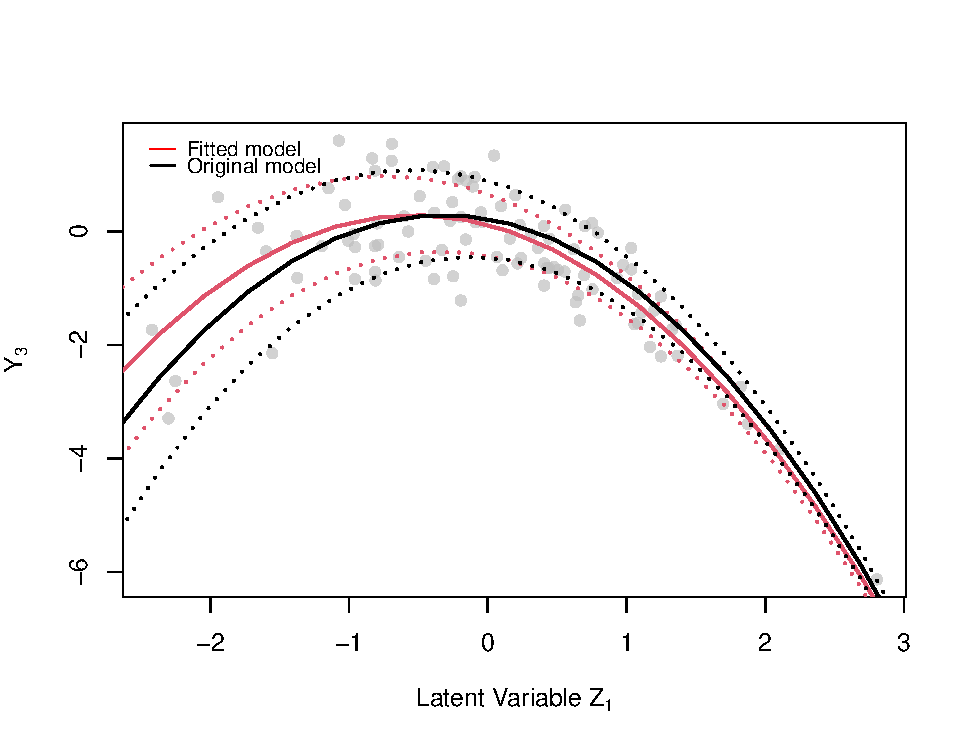
\includegraphics[width=\textwidth]{n100_GausHTQT}
    \caption{n = 100}
    \label{fig:Sim1n100}
\end{subfigure}
~ %add desired spacing between images, e. g. ~, \quad, \qquad, \hfill etc. 
  %(or a blank line to force the subfigure onto a new line)
\begin{subfigure}[b]{0.3\textwidth}
    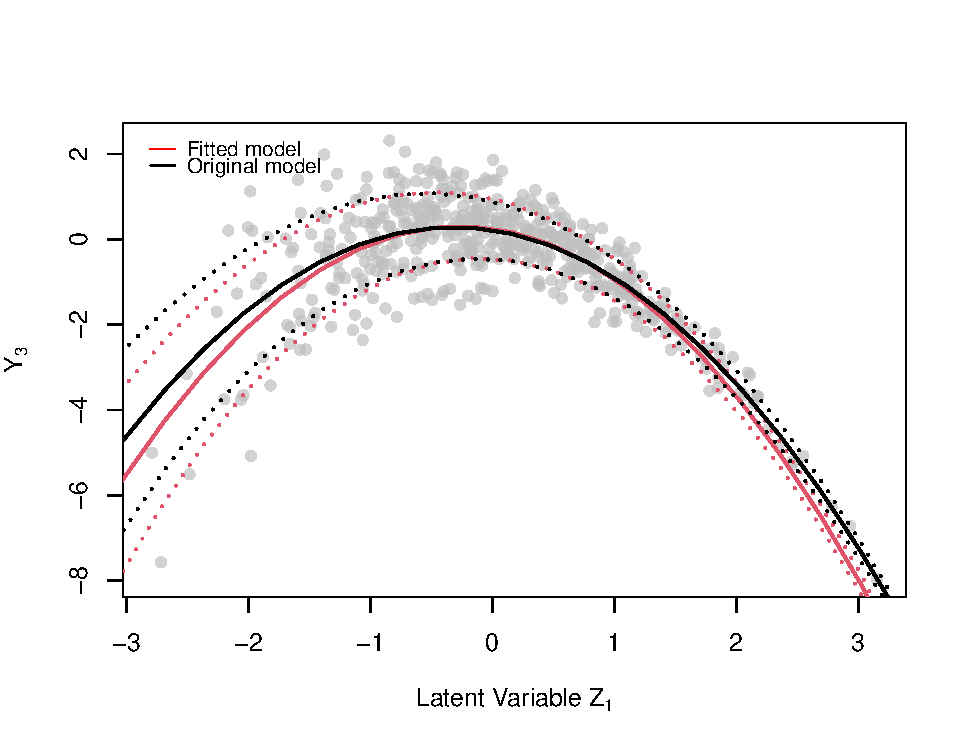
\includegraphics[width=\textwidth]{n500_GausQTHT}
    \caption{n = 500}
    \label{fig:Sim1n500}
\end{subfigure}
~ %add desired spacing between images, e. g. ~, \quad, \qquad, \hfill etc. 
%(or a blank line to force the subfigure onto a new line)
\begin{subfigure}[b]{0.3\textwidth}
    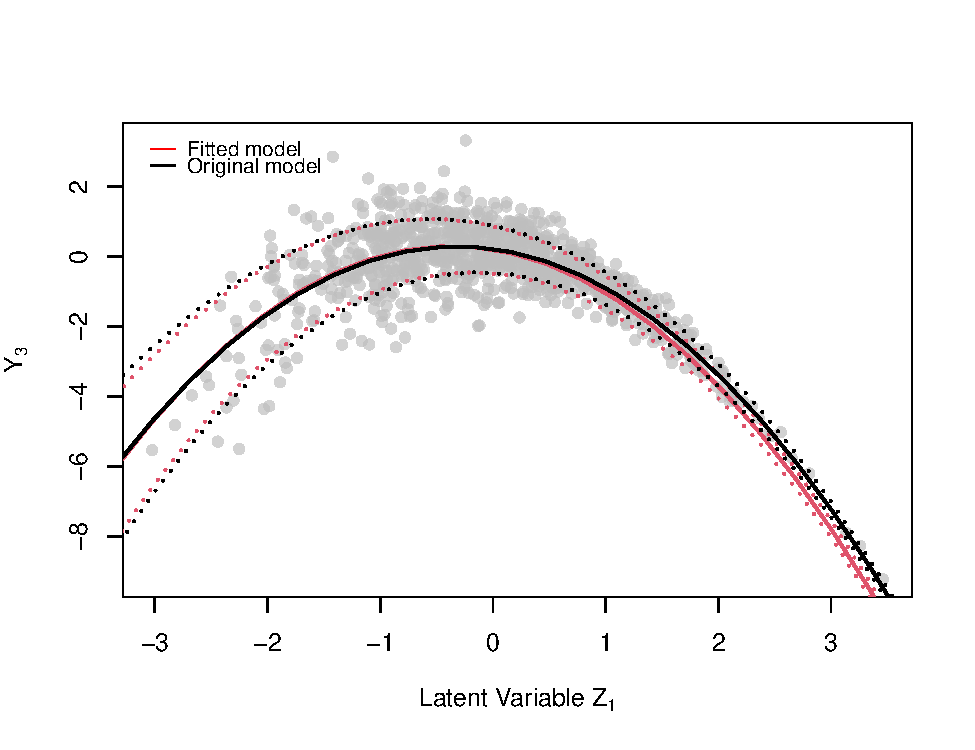
\includegraphics[width=\textwidth]{n1000_GausQTHT}
    \caption{n = 1000}
    \label{fig:Sim1n1000}
\end{subfigure}
\caption{Quadratic Heteroscedastic Factor Model (Item 3): Simulated and estimated distributions for different sample sizes.}\label{fig:Sim1}
\end{figure}

\subsection{IRT Model with Interactions}

In our second simulation study we consider binary items and a nonlinear measurement equation for the probability (location) parameter of the Bernoulli distribution. In particular, we include two latent variables and an interaction term between them. This model is similar to the one considered in \citet{Rizopoulos&Moustaki_BJMSP2008}. For a random sample of size $n$, the observed items are simulated as $y_{i} \cond \mathbf{z} \sim \text{Ber}(\pi_{i})$, where $\pi_i = \mathbb{P}(y_{i} = 1 \cond \mathbf{z})$, and the measurement equations are
\begin{align*}
\pi_i & = \frac{\exp\left(\alpha_{i0,\pi} + \alpha_{i1,\pi} z_1 + \alpha_{i2,\pi} z_2 + \alpha_{i3,\pi} z_1 \cdot z_2 \right)}{ 1 + \exp\left(\alpha_{i0,\pi} + \alpha_{i1,\pi} z_1 + \alpha_{i2,\pi} z_2 + \alpha_{i3,\pi} z_1 \cdot z_2 \right)}
\end{align*}

For this exercise we generate the parameters for the simulation from $\text{Unif}(-2,2)$ for each loading in the parameter vectors $\bm{\alpha}_{i,\pi} = (\alpha_{i0,\pi}, \alpha_{i1,\pi}, \alpha_{i2,\pi}, \alpha_{i3,\pi})'$. We simulate 1,000 data-sets, assuming the latent variables follows a multivariate standard normal distribution (i.e., uncorrelated latent variables). Our simulated sample size is of 1,000 units and 10 items. For each dimension in the latent variable manifold, we use 15 quadrature points to approximate the integrals in the E-step (a total of 225 quadrature points). Similarly, we initialize the EM algorithm with starting values being equal to the original parameters plus a random disturbance coming from $\text{Unif}(-0.1,0.1)$. The results presented in Table \ref{tab:A1Sim2} in the Appendix section also show low bias and root mean squared error (RMSE). Figure \ref{fig:Sim2} shows the simulated and estimated probability surfaces for items 2 and 6, respectively. The latter was the item with highest RMSE and RB. However, Figure \ref{fig:Sim2item6} shows that the resulting curve from the estimated parameters is not very different from the original (simulated).

\begin{figure}
\centering
\begin{subfigure}[b]{0.9\textwidth}
    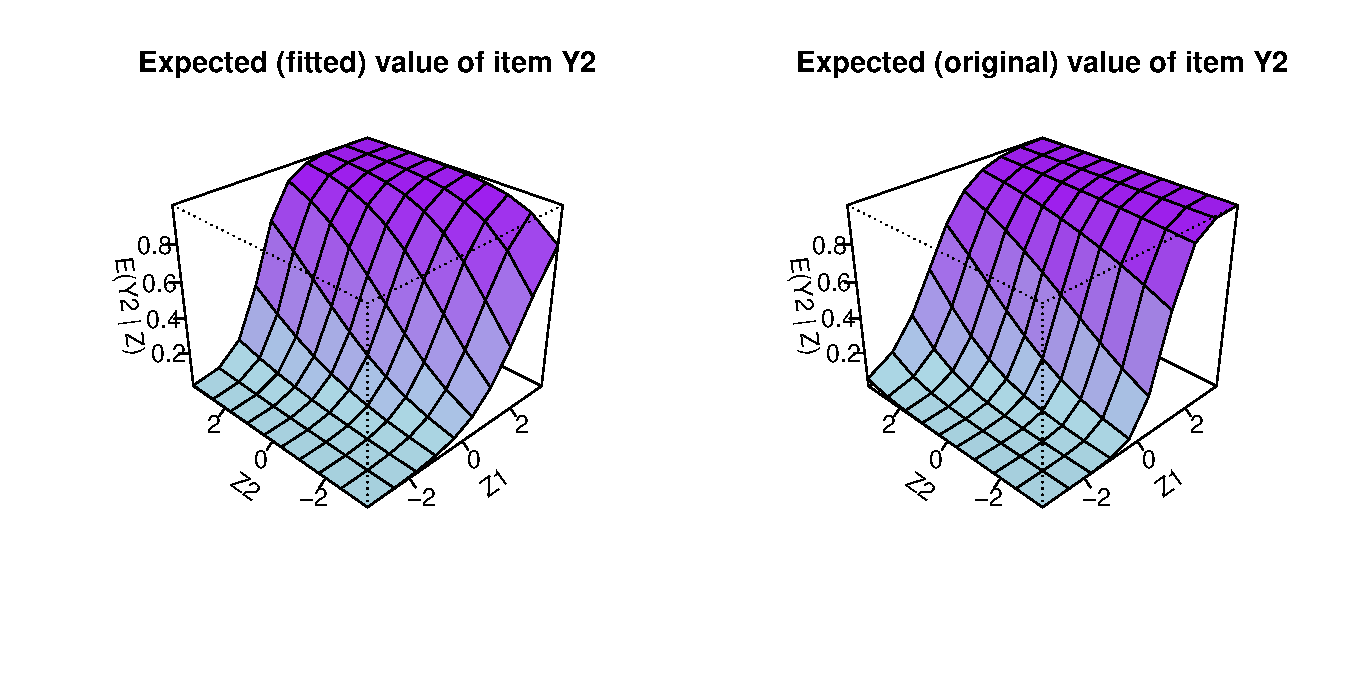
\includegraphics[width=\textwidth, trim = 0cm 2cm 2cm 0cm]{n1000_BernInt_item2.pdf}
    \caption{Item 2. True parameter values: $\alpha_{20,\pi} = -0.38;~\alpha_{21,\pi} = 1.92;~ \alpha_{22,\pi} = 0.51;~\alpha_{23,\pi} = -0.18$.}
    \label{fig:Sim2item2}
\end{subfigure}
\\ %add desired spacing between images, e. g. ~, \quad, \qquad, \hfill etc. 
  %(or a blank line to force the subfigure onto a new line)
\begin{subfigure}[b]{0.9\textwidth}
    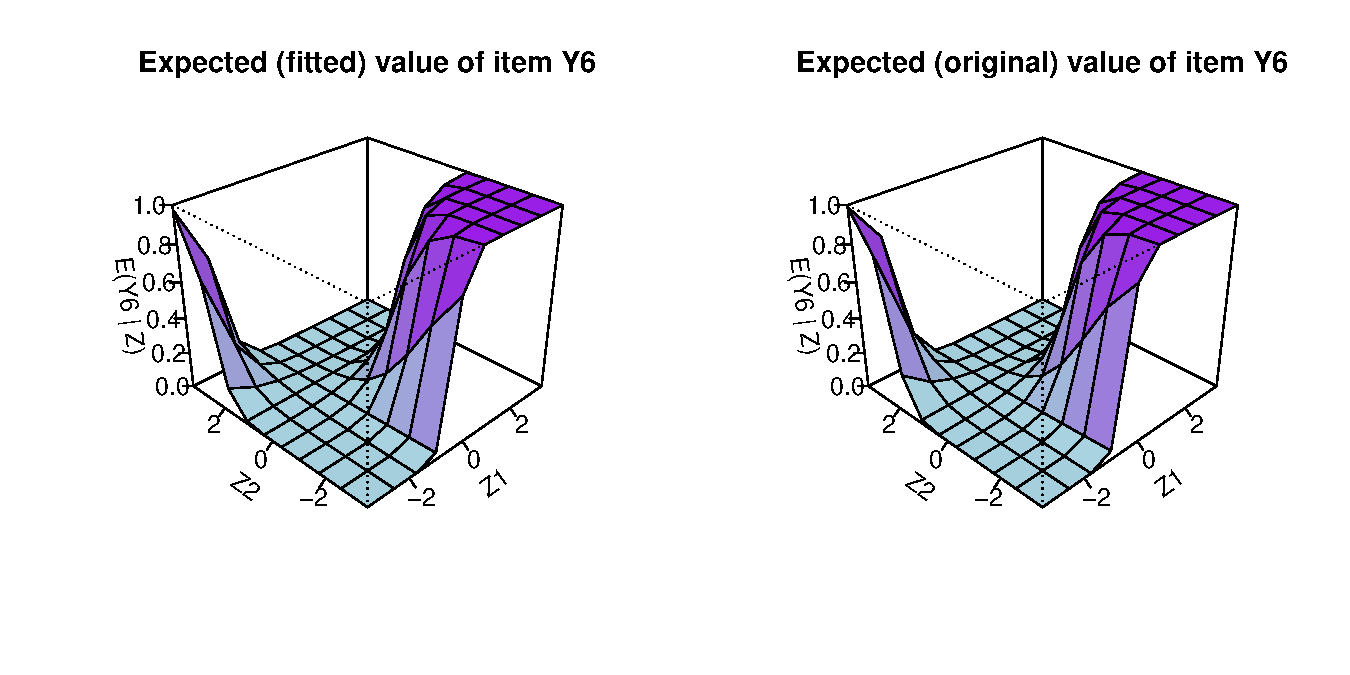
\includegraphics[width=\textwidth, trim = 0cm 2cm 2cm 0cm]{n1000_BernInt_item6.pdf}
    \caption{Item 6. True parameter values: $\alpha_{60,\pi} = -1.81;~\alpha_{61,\pi} = 1.63;~ \alpha_{62,\pi} = -1.76;~\alpha_{63,\pi} = -1.53$.}
    \label{fig:Sim2item6}
\end{subfigure}
\caption{Interaction IRT Model: Simulated and estimated probability surfaces for items 2 and 6.}\label{fig:Sim2}
\end{figure}

\subsection{Zero-Inflated Poisson Latent Variable Model}

In this example we estimate a Zero-Inflated Poisson latent variable model (ZIP-LVM), very similar to that in \citet{Wang_JoEdBS2010} and, to some extent, \citet{Hall_Biometrics2000}. More specifically, the distribution for the observed zero-inflated items (conditional on the latent variables $\mathbf{z}$), $f_i(y_i \cond \mathbf{z})$, is a mixture of a `perfect zero' process and a Poisson process, that is $y_i \cond \mathbf{z} \sim \text{ZIPois}(\lambda_i,\pi_i)$, with,
\begin{equation*}
y_i \cond \mathbf{z} \sim  
\begin{cases}
0, & \text{with probability } ~\pi_i \\
\text{Poisson}(\lambda_i), & \text{with probability } ~1-\pi_i
\end{cases}
\end{equation*}
which means that,
\begin{equation*}
f_i(y_{i} \cond \mathbf{z}) =
\begin{cases}
\pi_i + (1-\pi_i) \cdot e^{-\lambda_i}, & ~~\text{for } y_{i} = 0 \\[7pt]
(1-\pi_i) \cdot \dfrac{\lambda_i^{y_{i}} \cdot e^{-\lambda_i}}{y_{i}!}, & ~~\text{for } y_{i} = 1, 2, ...
\end{cases}
\end{equation*}

For ease of notation, we have avoided the dependency of the parameters $\lambda_i$ and $\pi_i$ on the latent variables $\mathbf{z}$. The probability distribution function above can be further expressed as 
\begin{equation*}
 f_i(y_{i} \cond \mathbf{z}) = \left(\pi_i + (1-\pi_i) \cdot e^{-\lambda_i}\right)^{u_{i}} \times \left((1-\pi_i) \cdot \dfrac{\lambda_i^{y_{i}} \cdot e^{-\lambda_i}}{y_{i}!}\right)^{(1-u_{i})},   
\end{equation*}

\noindent with $u_{i} = \mathbbm{1}_{\left\{y_i = 0\right\}}(y_{i})$ as an indicator function that equals 1 if $y_{i} = 0$ and 0 if $y_{i} > 0$. Our model extends that of \citet{Wang_JoEdBS2010} and \citet{Hall_Biometrics2000} as it allows for nonlinear functional forms on the link equations for $\lambda_i$ and $\pi_i$. In particular, in this simulation example we consider a quadratic measurement equation for the probability of an observation being sampled from the `pure zero' process. Using the semiparametric LVM notation, the measurement equations for the parameters $\lambda_i$ and $\pi_i$ in the ZIP-LVM are
\begin{align*}
\lambda_i & = \exp(\alpha_{i0,\lambda} + \alpha_{i1,\lambda} z_1) \\
\pi_i & = \frac{\exp(\alpha_{i0,\pi} + \alpha_{i1,\pi} z_1  + \alpha_{i2,\pi} z_1^2)}{1 + \exp(\alpha_{i0,\pi} + \alpha_{i1,\pi} z_1  + \alpha_{i2,\pi} z_1^2)}
\end{align*}

We generate 1,000 random samples of sizes $n$ = \{500, 1,000\}, for $p$ = 10 items. The parameter vectors  $\bm{\alpha}_{i,\lambda} = (\alpha_{i0,\lambda}, \alpha_{i1,\lambda})'$ and  $\bm{\alpha}_{i,\pi} = (\alpha_{i0,\pi}, \alpha_{i1,\pi}, \alpha_{i2,\pi})'$ were drawn from $\alpha_{i0,\lambda} \sim \text{Unif}(1,4)$; $\alpha_{i1,\lambda}, \alpha_{i0,\pi}, \alpha_{i1,\pi} \sim \text{Unif}(-1,1)$; and $\alpha_{i2,\pi} \sim \text{Unif}(-1.5,-0.5)$, Similarly, we initialize the EM algorithm with starting values being equal to the original parameters plus a random disturbance coming from $\text{Unif}(-0.1,0.1)$. One important limitation of this `incomplete' setting is that it is not clear whether an observation $m \in \{1,...,n\}$ was sampled from the `pure zero' state or from the Poisson state. Fortunately, LVM are already problems of missing data. Apart from the latent variables $\mathbf{z}$, the additional missing data in this problem is the vector of indicator variables $\mathbf{b}_i = (b_{i1},...,b_{in})'$, where $b_{im} = 1$ if $y_{im}= 0$ is from the `pure zero' state and $b_{im} = 0$ otherwise. Building on the `incomplete' data log-likelihood in equation \eqref{eq:logLik}, the `complete' log-likelihood for the ZIP-LVM can be written as
\begin{align*}
\mathcal{L}^c(\Theta; \mathbf{y}, \mathbf{b}) = & \sum\limits_{m=1}^n \log f^\text{c}(\mathbf{y}_m, \mathbf{b}_m) \\
= & \sum\limits_{m=1}^n \Big( \log f^c(\mathbf{y}_m \cond \mathbf{b}_m) + \log p(\mathbf{b}_m) \Big) \\
= & \sum\limits_{m=1}^n \left( \log \left[ \int_{\R^q} \prod\limits_{i=1}^p f^c_i(y_{im} \cond b_{im}, \mathbf{z}) ~ p(\mathbf{z}) ~ \text{d}\mathbf{z} \right] + \log \left[ \int_{\R^q} \prod\limits_{i=1}^p p_i(b_{im} \cond \mathbf{z}) ~ p(\mathbf{z}) ~ \text{d}\mathbf{z} \right] \right) \\
= & \sum\limits_{m=1}^n \log \left[ \int_{\R^q} \prod\limits_{i=1}^p \left(\dfrac{\lambda_{im}^{y_{im}} \cdot e^{-\lambda_{im}}}{y_{im}!}\right)^{(1-b_{im})} ~ p(\mathbf{z}) ~ \text{d}\mathbf{z} \right] + \\
& \sum\limits_{m=1}^n \log \left[ \int_{\R^q} \prod\limits_{i=1}^p \left(\pi_{im}^{b_{im}} \cdot (1-\pi_{im})^{(1-b_{im})}\right) ~ p(\mathbf{z}) ~ \text{d}\mathbf{z} \right] =  \mathcal{L}^c_1(\Theta; \mathbf{y}, \mathbf{b}) + \mathcal{L}^c_2(\Theta; \mathbf{b}) %\\[5pt] 
\end{align*}

This log-likelihood is easy to maximize, because $\mathcal{L}^c_1(\Theta; \mathbf{y}, \mathbf{b})$ and $\mathcal{L}^c_2(\Theta; \mathbf{b})$ can be maximized separately. When solving for the ML estimates of $\Theta$, both components of the complete log-likelihood, $\mathcal{L}^c_1(\Theta; \mathbf{y}, \mathbf{b})$ and $\mathcal{L}^c_2(\Theta; \mathbf{b})$, become linear with respect to $\mathbf{b}$. This feature allows for a straightforward adaptation of the EM algorithm to include the vector of missing data $\mathbf{b}$. Indeed, the E-step of the EM algorithm requires computing the expectation of the `complete' log-likelihood with respect to the joint distribution of the missing data, $(\mathbf{z},\mathbf{b})$, as %$\mathbb{E}_{(\mathbf{z},\mathbf{b})} [\!~ \mathcal{L}^c(\Theta; \mathbf{y}, \mathbf{b})\!~]$, as
\begin{align*}
\mathbb{E}_{(\mathbf{z},\mathbf{b})}\left[\!~ \mathcal{L}^c(\Theta; \mathbf{y},\mathbf{b}) \!~\right] = &~ \mathbb{E}_{(\mathbf{z},\mathbf{b})} \left[\!~ \mathcal{L}^c_1(\Theta; \mathbf{y},\mathbf{b}) \!~\right] + \mathbb{E}_{(\mathbf{z},\mathbf{b})} \left[\!~ \mathcal{L}^c_2(\Theta; \mathbf{b}) \!~\right] \\
= &~ \mathbb{E}_{\mathbf{z}} \left[\!~ \mathbb{E}_{\mathbf{b}} \left[\!~ \mathcal{L}^c_1(\Theta; \mathbf{y},\mathbf{b}) \!~\right] \!~\right] +  \mathbb{E}_{\mathbf{z}} \left[\!~ \mathbb{E}_{\mathbf{b}} \left[\!~ \mathcal{L}^c_2(\Theta; \mathbf{b}) \!~\right] \!~\right]
\end{align*}

Since both double-expectations above are linear with respect to $\mathbf{b}$, the inner expectations with respect to $\mathbf{b}$ become $\mathcal{L}_1^c(\Theta; \mathbf{y}, \bar{\mathbf{b}})$ and $\mathcal{L}_2^c(\Theta; \bar{\mathbf{b}})$, where $\bar{\mathbf{b}} = (\bar{\mathbf{b}}_1',...,\bar{\mathbf{b}}_p')'$ and $\bar{\mathbf{b}}_i = (\bar{b}_{i1},...,\bar{b}_{in})'$ for $i=1,...,p$, and with the the expected value of $\bar{b}_{im} = \mathbb{E}_\mathbf{b}(b_{im} \cond y_{im}, \mathbf{z}_m, \Theta)$, defined as
\begin{align*}
\mathbb{E}_\mathbf{b}(b_{i} \cond y_{i}, \mathbf{z}, \Theta) = & ~ \mathbb{P}(b_{i} = 1 \cond y_{i}, \mathbf{z}, \Theta)\\
= & ~ \frac{f_i^c(y_{i} \cond b_i = 1, \mathbf{z}, \Theta) \cdot p_i(b_{i} = 1 \cond \mathbf{z}, \Theta)} {f_i^c(y_{i} \cond b_i = 1, \mathbf{z}, \Theta) \cdot p_i(b_{i} = 1 \cond \mathbf{z}, \Theta) + f_i^c(y_{i} \cond b_i = 0, \cond \mathbf{z}, \Theta) \cdot p_i(b_{i} = 0 \cond \mathbf{z}, \Theta)} \\[5pt]
= & ~ \begin{cases}
\left[1 + \exp(-\text{logit}(\pi_i) - \lambda_i) \right]^{-1}, & \text{if ~} y_i = 0 \\
0, & \text{if ~} y_i > 0
\end{cases}
\end{align*}
where $\lambda_i$ and $\pi_i$ are nonlinear functions of $\mathbf{z}$ with parameters $\Theta$. Having replaced $\bar{\mathbf{b}}$ inside the inner expectations above, the outer expectations, $\mathbb{E}_{\mathbf{z}}\left[\!~\mathcal{L}_1^c(\Theta; \mathbf{y}, \bar{\mathbf{b}}) \!~\right]$ and $\mathbb{E}_{\mathbf{z}} \left[\!~\mathcal{L}_2^c(\Theta; \bar{\mathbf{b}})\!~\right]$ can be computed using the Gaussian Quadrature rule described in the Appendix. The M-step can be carried as usual. The simulation results presented in Table \ref{tab:A1Sim3} the Appendix section show low bias and root mean squared error (RMSE).


\section{Factor scores}

\section{Empirical application}

\section{Final remarks}

\setcounter{table}{0}
\setcounter{algorithm}{0}
\setcounter{figure}{0}
\renewcommand{\thetable}{A\arabic{table}}
\renewcommand{\thealgorithm}{A\arabic{algorithm}}
\renewcommand{\thefigure}{A\arabic{figure}}

\section{Appendix}

\subsection{Maximum Likelihood (ML) Estimation}

Consider the likelihood function in equation \eqref{eq:logLik}. For simplicity, assume a parametric function (linear or nonlinear, but of known form) for the measurement equations $g_{i,\varphi}(\cdot)$ in \eqref{eq:genLVMmu} to \eqref{eq:genLVMtau}. Given a random sample of $n$ independent units, and under the assumption of conditional independence, the log-likelihood of the manifest variables is:
\begin{align*}
\mathcal{L}(\Theta; \mathbf{y}) = \sum_{m=1}^{n} \log f(\mathbf{y}_m) & = \sum_{m=1}^{n} \log \left[\int_{\R^q} f(\mathbf{y}_m \cond \mathbf{z})~ p(\mathbf{z}) ~ \text{d}\mathbf{z}\right] \nonumber \\ & = \sum_{m=1}^{n} \log \left[\int_{\R^q} \prod_{i=1}^p f_i(y_{im} \cond \mathbf{z}) ~ p(\mathbf{z}) ~ \text{d}\mathbf{z}\right]
\end{align*}

where $\Theta = \mathrm{vech}(\bm{\alpha}_{i,\varphi})$ is the vector of all the model parameters (intercepts and slopes) for the parameters in the density functions of the observed items, that is $\varphi_i \in \theta_i = \{\mu_i, \sigma_i, \tau_i, \nu_i\}$, for every $i = 1,...,p$. The subscript in $\bm{\theta}_m$ refers to a particular unit $m$ in our sample, such that $\bm{\theta}_m = (\theta_{1m},...,\theta_{pm})'$, where $\theta_{im} = (\mu_{im}, \sigma_{im}, \nu_{im}, \tau_{im})'$, and every parameter in $\theta_{im}$ is a (nonlinear) function of $\mathbf{z}_{m}$.

First, we derive a general expression for the first derivative of the log-likelihood above with respect to the parameters in $\Theta$. Let $\mathbb{S} = \mathrm{vec}(\mathbb{S}_{i,\varphi})$ be the stacked vector of first derivatives of the log-likelihood with respect to the column vector of loadings $\bm{\alpha}_{i,\varphi}$ for each item $i = 1,...,p$ and each parameter $\varphi \in \theta_i$. Avoiding the dependence on $\bm{\theta}_m$ in the likelihood functions (for notational simplicity), $\mathbb{S}_{i,\varphi}$ takes the form:
\begin{align*}
\mathbb{S}_{i,\varphi} = \frac{\partial \mathcal{L}(\Theta; \mathbf{y})}{\partial \bm{\alpha}_{i,\varphi}} & = \sum\limits_{m=1}^{n} \frac{1}{f(\mathbf{y}_m)} \cdot \left[ \int_{\R^q} \frac{f(\mathbf{y}_m \cond \mathbf{z}) p(\mathbf{z})}{f_i(y_{im} \cond \mathbf{z})} \cdot \frac{\partial}{\partial \bm{\alpha}_{i,\varphi}} f_i(y_{im} \cond \mathbf{z}) ~ \text{d}\mathbf{z} \right] \\[3mm]
& = \sum\limits_{m=1}^{n} \int_{\R^q} p(\mathbf{z} \cond \mathbf{y}_m) \cdot \frac{\partial}{\partial \bm{\alpha}_{i,\varphi}} \log f_i(y_{im} \cond \mathbf{z}) ~ \text{d}\mathbf{z} \label{eq:A1score} \tag{A1} \\[3mm]
& = \sum\limits_{m=1}^{n} \int_{\R^q} p(\mathbf{z} \cond \mathbf{y}_m) \cdot \frac{\partial \log f_i(y_{im} \cond \mathbf{z})}{ \partial \varphi_i} \cdot \frac{\partial \varphi_i}{\partial \eta_{i,\varphi}} \cdot \frac{\partial \eta_{i,\varphi}}{\partial \bm{\alpha}_{i,\varphi}}~ \text{d}\mathbf{z} ; 
\end{align*}

where $p(\mathbf{z} \cond \mathbf{y}_m)$ is the posterior density of the latent variables, and the partial derivatives with respect to $\varphi_i$, $\eta_{i,\varphi}$, and $\bm{\alpha}_{i,\varphi}$ depend on the density function for the item $i$, $f_i$; the inverse of the link function, $\upsilon_{i,\varphi}(\varphi_i)$; and the (nonlinear) parametric form for $\eta_{i,\varphi}$ on $\mathbf{z}$, respectively. Analytical expressions for all of the above are presented separately in Appendices \ref{sec:AppAnalytical} and \ref{sec:AppLink}.

The estimates of the parameters in $\Theta$ that directly maximize the log-likelihood in equation \eqref{eq:logLik} are the ones that solve for the system of equations $\mathbb{S}_{i,\varphi} = 0$, for each $\varphi_i \in \theta_i$ in $i = 1,...,p$. Denote the aforementioned vector as $\hat{\Theta}$. In most cases, there is no analytical solution to these score equations and must be solved using numerical approximations, such as the iterative Newton-Raphson algorithm or trust region alternatives. Numerical methods often use second order approximations to the function of interest, requiring the computation of the matrix of second derivatives (known as the Hessian matrix). Let $\mathbb{H}$ be a squared, symmetric matrix composed of the sub-matrices of second derivatives of the observed data log-likelihood, $\mathbb{H}_{(j,\tilde{\varphi})}^{(i,\varphi)}$ for each $(\varphi, \tilde{\varphi}) \in \theta$ and $i,j \in \{1,...,p\}$. These matrices take the form:
\begin{equation*}
\mathbb{H}_{(j,\tilde{\varphi})}^{(i,\varphi)} =  \frac{\partial^2 \mathcal{L}(\Theta; \mathbf{y})}{\partial \bm{\alpha}_{i,\varphi} \partial \bm{\alpha}'_{j,\tilde{\varphi}}} = \frac{\partial \mathbb{S}_{i,\varphi}}{\partial \bm{\alpha}'_{j,\tilde{\varphi}}}
\end{equation*}
that is,
\begin{align*}
\mathbb{H}_{(j,\tilde{\varphi})}^{(i,\varphi)} & = \sum\limits_{m=1}^{n} \int_{\R^q} \left[p(\mathbf{z} \cond \mathbf{y}_m) \cdot \frac{\partial^2 \log f_i(y_{im} \cond \mathbf{z})}{\partial \bm{\alpha}_{i,\varphi} \partial \bm{\alpha}'_{j,\tilde{\varphi}}} + \frac{\partial \log f_i(y_{im} \cond \mathbf{z})}{\partial \bm{\alpha}_{i,\varphi}} \cdot \underbrace{\frac{\partial p(\mathbf{z} \cond \mathbf{y}_m)}{\partial \bm{\alpha}'_{j,\tilde{\varphi}}}}_{\mathbb{H}1'} \right] ~ \text{d}\mathbf{z}; \label{eq:A2Hessian} \tag{A2}
\end{align*}

where the transposed vector $\mathbb{H}1$ in the integrand above is computed as

\begin{align*}
\mathbb{H}1 = & ~ \frac{\partial p(\mathbf{z} \cond \mathbf{y}_m)}{\partial \bm{\alpha}_{j,\tilde{\varphi}}} = \frac{\partial}{\partial \bm{\alpha}_{j,\tilde{\varphi}}} \left[ \frac{f(\mathbf{y}_m \cond \mathbf{z}) p(\mathbf{z})}{f(\mathbf{y}_m)} \right] \\[3mm]
= & ~ \frac{\partial}{\partial \bm{\alpha}_{j,\tilde{\varphi}}} \left[ \frac{f(\mathbf{y}_m \cond \mathbf{z}) p(\mathbf{z})}{\int_{\R^q} f(\mathbf{y}_m \cond \mathbf{z}) p(\mathbf{z})~ \text{d}\mathbf{z}} \right]\\[3mm]
= & ~ \frac{\left[\dfrac{\partial f(\mathbf{y}_m \cond \mathbf{z}) p(\mathbf{z})}{\partial \bm{\alpha}_{j,\tilde{\varphi}}} \cdot \int_{\R^q} f(\mathbf{y}_m \cond \mathbf{z}) p(\mathbf{z}) ~ \text{d}\mathbf{z} \right] - \left[ \dfrac{\partial\left(\int_{\R^q} f(\mathbf{y}_m \cond \mathbf{z}) p(\mathbf{z}) ~ \text{d}\mathbf{z} \right)}{\partial \bm{\alpha}_{j,\tilde{\varphi}}} \cdot f(\mathbf{y}_m \cond \mathbf{z}) p(\mathbf{z}) \right]} {\left[ \int_{\R^q} f(\mathbf{y}_m \cond \mathbf{z}) p(\mathbf{z})~ \text{d}\mathbf{z} \right]^2} \\[3mm]
= & ~ \frac{f(\mathbf{y}_m \cond \mathbf{z}) p(\mathbf{z})}{\int_{\R^q} f(\mathbf{y}_m \cond \mathbf{z}) p(\mathbf{z})~ \text{d}\mathbf{z}} \cdot 
\left[ \frac{\partial f(\mathbf{y}_m \cond \mathbf{z}) p(\mathbf{z})}{\partial \bm{\alpha}_{j,\tilde{\varphi}}} \frac{1}{f(\mathbf{y}_m \cond \mathbf{z}) p(\mathbf{z})} \right]\\[3mm]
& ~ - \frac{f(\mathbf{y}_m \cond \mathbf{z}) p(\mathbf{z})}{\int_{\R^q} f(\mathbf{y}_m \cond \mathbf{z}) p(\mathbf{z})~ \text{d}\mathbf{z}} \cdot 
\left[{\displaystyle \int_{\R^q}} \frac{\partial f(\mathbf{y}_m \cond \mathbf{z}) p(\mathbf{z})}{\partial \bm{\alpha}_{j,\tilde{\varphi}}} \frac{1}{f(\mathbf{y}_m \cond \mathbf{z}) p(\mathbf{z})}~ \text{d}\mathbf{z} \cdot \frac{f(\mathbf{y}_m \cond \mathbf{z}) p(\mathbf{z})}{\int_{\R^q} f(\mathbf{y}_m \cond \mathbf{z}) p(\mathbf{z})~ \text{d}\mathbf{z}} 
\right] \\[3mm]
= & ~ p(\mathbf{z} \cond \mathbf{y}_m) \cdot \frac{\partial}{\partial \bm{\alpha}_{j,\tilde{\varphi}}} \log f(\mathbf{y}_m \cond \mathbf{z}) - ~ p(\mathbf{z} \cond \mathbf{y}_m) \cdot \left[\int_{\R^q} p(\mathbf{z} \cond \mathbf{y}_m) \frac{\partial}{\partial \bm{\alpha}_{j,\tilde{\varphi}}} \log f(\mathbf{y}_m \cond \mathbf{z}) ~\text{d}\mathbf{z} \right] \\[3mm]
= & ~  p(\mathbf{z} \cond \mathbf{y}_m) \cdot \frac{\partial}{\partial \bm{\alpha}_{j,\tilde{\varphi}}} \log f_j(y_{jm} \cond \mathbf{z}) - ~ p(\mathbf{z} \cond \mathbf{y}_m) \cdot \left[\int_{\R^q} p(\mathbf{z} \cond \mathbf{y}_m) \frac{\partial}{\partial \bm{\alpha}_{j,\tilde{\varphi}}} \log f_j(y_{jm} \cond \mathbf{z}) ~\text{d}\mathbf{z} \right]
\end{align*}

With the above, equation \eqref{eq:A2Hessian} becomes

\begin{align*}
\mathbb{H}_{(j,\tilde{\varphi})}^{(i,\varphi)} & =  \sum\limits_{m=1}^{n} \int_{\R^q} p(\mathbf{z} \cond \mathbf{y}_m) \cdot \frac{\partial^2 \log f_i(y_{im} \cond \mathbf{z})}{\partial \bm{\alpha}_{i,\varphi} \partial \bm{\alpha}'_{j,\tilde{\varphi}}} ~ \text{d}\mathbf{z} \\[3mm]
& + \sum\limits_{m=1}^{n} \int_{\R^q} p(\mathbf{z} \cond \mathbf{y}_m) \cdot \frac{\partial \log f_i(y_{im} \cond \mathbf{z})}{\partial \bm{\alpha}_{i,\varphi}} \cdot \frac{\partial \log f_j(y_{jm} \cond \mathbf{z})}{\partial \bm{\alpha}'_{j,\tilde{\varphi}}} ~ \text{d}\mathbf{z} \\[3mm]
& - \sum\limits_{m=1}^{n} \int_{\R^q} p(\mathbf{z} \cond \mathbf{y}_m) \cdot \frac{\partial \log f_i(y_{im} \cond \mathbf{z})}{\partial \bm{\alpha}_{i,\varphi}} ~ \text{d}\mathbf{z} \cdot \int_{\R^q} p(\mathbf{z} \cond \mathbf{y}_m) \frac{\partial  \log f_j(y_{jm} \cond \mathbf{z})}{\partial \bm{\alpha}'_{j,\tilde{\varphi}}} ~\text{d}\mathbf{z} \label{eq:A3Hessian2} \tag{A3}
\end{align*}

Note that the matrix of second derivatives in the first summation can be expressed as
\begin{equation*}
\frac{\partial^2 \log f_i(y_{im} \cond \mathbf{z})}{\partial \bm{\alpha}_{i,\varphi} \partial \bm{\alpha}'_{j,\tilde{\varphi}}} = \frac{\partial \eta_{i,\varphi}}{\partial \bm{\alpha}_{i,\varphi}} \cdot  \frac{\partial \varphi_i}{\partial \eta_{i,\varphi}} \cdot \frac{\partial^2 \log f_i(y_{im} \cond \mathbf{z})}{ \partial \varphi_i \partial \tilde{\varphi}_j} \cdot \frac{\partial \tilde{\varphi}_j}{\partial \eta_{j,\tilde{\varphi}}} \cdot \frac{\partial \eta_{j,\tilde{\varphi}}}{\partial \bm{\alpha}'_{j,\tilde{\varphi}}}, 
\end{equation*}
and that the last summation in the expression above is simply $\mathbb{S}_{i,\varphi} \cdot \mathbb{S}'_{j,\tilde{\varphi}}$. In general, but in particular for complex models, the Hessian matrix can be computationally intensive to compute. In these cases, it is easier to find good approximations by computing and using their expected value instead, $\mathbb{E}_{\mathbf{y}}(\mathbb{H}^{(i,\varphi)}_{(j,\tilde{\varphi})}) = \mathcal{H}^{(i,\varphi)}_{(j,\tilde{\varphi})}$. For this purpose, we shall assume a reasonably large sample size. This matrix, known as the expected Fisher information matrix, takes the form
%\begin{align*}
%\mathcal{S}_{i,\varphi} = \mathbb{E}(\mathbb{S}_{i,\varphi}) & = \mathbb{E}\left(\frac{\partial \mathcal{L}(\Theta; \mathbf{y})}{\partial \bm{\alpha}_{i,\varphi}} \right) = \int_{\R^p} \frac{\partial \mathcal{L}(\Theta; \mathbf{y})}{\partial \bm{\alpha}_{i,\varphi}} f(\mathbf{y}) ~\text{d}\mathbf{y} \\[3mm]
%& = \int_{\R^p} \frac{\partial \log f(\mathbf{y})}{\partial \bm{\alpha}_{i,\varphi}} f(\mathbf{y}) ~\text{d}\mathbf{y} = \int_{\R^p} \frac{1}{f(\mathbf{y})} \frac{\partial f(\mathbf{y})}{\partial \bm{\alpha}_{i,\varphi}} f(\mathbf{y}) ~ \text{d}\mathbf{y} \\[3mm]
%& = \frac{\partial}{\partial \bm{\alpha}_{i,\varphi}} \int_{\R^p} f(\mathbf{y}) ~\text{d}\mathbf{y} = \frac{\partial}{\partial \bm{\alpha}_{i,\varphi}} 1 = \vec{0}
%\end{align*}
%and
\begin{align*}
\bm{0} = \frac{\partial}{\partial \bm{\alpha}'_{j,\tilde{\varphi}}} \mathbb{E}_{\mathbf{y}}\left[\mathbb{S}_{i,\varphi}\right] = & ~ \frac{\partial }{\partial \bm{\alpha}'_{j,\tilde{\varphi}}} \int_{\R^p} \frac{\partial \log f(\mathbf{y})}{\partial \bm{\alpha}_{i,\varphi}} f(\mathbf{y}) ~\text{d}\mathbf{y} = \int_{\R^p} \frac{\partial}{\partial \bm{\alpha}'_{j,\tilde{\varphi}}} \left\{ \frac{\partial \log f(\mathbf{y})}{\partial \bm{\alpha}_{i,\varphi}} f(\mathbf{y}) \right\} ~\text{d}\mathbf{y} \\[3mm]
= & ~ \int_{\R^p} \left\{ \frac{\partial^2 \log f(\mathbf{y})}{\partial \bm{\alpha}_{i,\varphi} \partial \bm{\alpha}'_{j,\tilde{\varphi}}} f(\mathbf{y}) + \frac{\partial \log f(\mathbf{y})}{\partial \bm{\alpha}_{i,\varphi}} \frac{\partial f(\mathbf{y})}{\partial \bm{\alpha}'_{j,\tilde{\varphi}}} \right\} ~\text{d}\mathbf{y} \\[3mm]
= & ~ \int_{\R^p} \frac{\partial^2 \log f(\mathbf{y})}{\partial \bm{\alpha}_{i,\varphi} \partial \bm{\alpha}'_{j,\tilde{\varphi}}} f(\mathbf{y}) ~\text{d}\mathbf{y} + \int_{\R^p} \frac{\partial \log f(\mathbf{y})}{\partial \bm{\alpha}_{i,\varphi}} \frac{\partial \log f(\mathbf{y})}{\partial \bm{\alpha}'_{j,\tilde{\varphi}}} f(\mathbf{y}) ~\text{d}\mathbf{y} \\[3mm]
= & ~ \mathbb{E}_{\mathbf{y}}\left[\frac{\partial^2 \log f(\mathbf{y})}{\partial \bm{\alpha}_{i,\varphi} \partial \bm{\alpha}'_{j,\tilde{\varphi}}} \right] +  \mathbb{E}_{\mathbf{y}}\left[\frac{\partial \log f(\mathbf{y})}{\partial \bm{\alpha}_{i,\varphi}} \frac{\partial \log f(\mathbf{y})}{\partial \bm{\alpha}'_{j,\tilde{\varphi}}} \right] \\[3mm]
= & ~ \mathbb{E}_{\mathbf{y}}\left[\mathbb{H}^{(i,\varphi)}_{(j,\tilde{\varphi})}\right] + \mathbb{E}_{\mathbf{y}}\left[\mathbb{S}_{i,\varphi} \mathbb{S}'_{j,\tilde{\varphi}}\right] \\[3mm]
\Longrightarrow & ~ \mathcal{H}^{(i,\varphi)}_{(j,\tilde{\varphi})} = \mathbb{E}_{\mathbf{y}}\left[\mathbb{H}^{(i,\varphi)}_{(j,\tilde{\varphi})}\right] = - \mathbb{E}_{\mathbf{y}}\left[\mathbb{S}_{i,\varphi} \mathbb{S}'_{j,\tilde{\varphi}}\right]
\end{align*}

\subsection{ML estimation using the EM algorithm}

Recall that in most cases, there is no closed form expression for  $\mathbb{S}_{i,\varphi} = 0$, and that we need to apply numerical methods to find solve for $\hat{\Theta}$. Apart from this inconvenience, when solving the score equations we run into the problem of dealing with latent variables (i.e., non-observed data). We resort to the Expectation-Maximization (EM, \citealp{DempsterEtAl_JRSS1977, Bock&Aitkin_Psychometrika1981}) algorithm, a popular tool in the estimation of models with missing data (in addition to the unknown parameters of the model). This procedure allows for an efficient ML estimation of the parameters in the Generalized Latent Variable Model (GLVM) framework, a case in which for most distributional cases there are no closed form solutions for the score equations.

In general terms, the implementation of the EM algorithm consists of two iterative steps when trying to find the parameter estimates $\hat{\Theta}$ that maximize the log-likelihood function of the observed data $\mathcal{L}(\mathbf{y};\Theta)$. First, for every $t$\textsuperscript{th} iteration, the `Expectation' step (E-step) requires taking the expected value of the observed log-likelihood with respect to the posterior distribution of the latent variables $\mathbf{z}$ given $\mathbf{y}$ and the current estimates of the parameters $\Theta^{[t]}$, as
\begin{equation*}
\mathcal{Q}(\Theta;\Theta^{[t]}) = \mathbb{E}_{\mathbf{z} \cond \mathbf{y}, \Theta^{[t]}}\left[\!~\mathcal{L}(\Theta; \mathbf{y})\!~\right]
\end{equation*}
Secondly, in the `Maximization' step (M-step), we update the parameters estimates to maximize the quantity above, as
\begin{equation*}
\Theta^{[t+1]} = \argmax \mathcal{Q}(\Theta;\Theta^{[t]})
\end{equation*}

We explain in detail the EM steps below, and with detail in Algorithm \ref{alg:EMalg}:

\paragraph{E-step:} The values that maximize the objective function are those that solve for the equations $\partial \mathcal{Q} / \partial \Theta = 0$. Note that Leibniz integral rule allows for expressing the gradient of $\mathcal{Q}$  as
\begin{equation*}
\dfrac{\partial}{\partial \Theta} \mathbb{E}_{\mathbf{z} \cond \mathbf{y}, \Theta^{[t]}} \left[\!~\mathcal{L}(\Theta; \mathbf{y})\!~\right] = \mathbb{E}_{\mathbf{z} \cond \mathbf{y}, \Theta^{[t]}} \left[\!~\dfrac{\partial}{\partial \Theta} \mathcal{L}(\Theta; \mathbf{y})\!~\right] = \mathbb{E}_{\mathbf{z} \cond \mathbf{y}, \Theta^{[t]}} \left[\!~\mathbb{S} \!~\right]
\end{equation*}

We can evaluate the expected value above separately for each vector $\mathbb{S}_{i,\varphi} \in \mathbb{S}$, and thus, from equation \eqref{eq:A1score} we can see that 
\begin{align*}
\mathbb{E}_{\mathbf{z}\cond \mathbf{y},\bm{\alpha}_{i,\varphi}} \left[\!~ \mathbb{S}_{i,\varphi}\!~\right] & = \sum\limits_{m = 1}^{n} \mathbb{E}_{\mathbf{z}\cond \mathbf{y},\bm{\alpha}_{i,\varphi}} \left[\!~ \int_{\R^q} p(\mathbf{z} \cond \mathbf{y}_m) \cdot \frac{\partial}{\partial \bm{\alpha}_{i,\varphi}} \log f_i(y_{im} \cond \mathbf{z}) ~ \text{d}\mathbf{z} \!~\right] \\
& = \sum\limits_{m = 1}^{n} \mathbb{E}_{\mathbf{z}\cond \mathbf{y},\bm{\alpha}_{i,\varphi}} \left[\!~  \mathbb{E}_{\mathbf{z}\cond \mathbf{y},\bm{\alpha}_{i,\varphi}} \left[\!~  \frac{\partial}{\partial \bm{\alpha}_{i,\varphi}} \log f_i(y_{im} \cond \mathbf{z}) \!~\right] \!~\right] \\
& =  \sum\limits_{m = 1}^{n} \mathbb{E}_{\mathbf{z}\cond \mathbf{y},\bm{\alpha}_{i,\varphi}} \left[\!~  \frac{\partial}{\partial \bm{\alpha}_{i,\varphi}} \log f_i(y_{im} \cond \mathbf{z}) \!~\right] = \mathbb{S}_{i,\varphi}
\end{align*}

From the above it can be seen that the E-step is attained by simply computing the integrals in the score equations $\mathbb{S}_{i,\varphi}$, for every $\varphi \in \theta_i$ and $i = 1,...,p$. These integrals over the latent variables $\mathbf{z} \in \R^q$ are difficult (if not tedious) to evaluate analytically. As it is common in the LVM literature, and following \citet{Rizopoulos&Moustaki_BJMSP2008}, we use a multivariate Gaussian-Hermite quadrature to numerically approximate of the q-dimensional integrals of the form
\begin{equation*}
\int_{\R^q} \exp(-\mathbf{z}'\mathbf{z}) f(\mathbf{z}) ~\text{d}\mathbf{z} \approx \sum\limits_{r_1 = 1}^{R_1} \cdots \sum\limits_{r_q = 1}^{R_q} w_{r_1} \cdots w_{r_q} f(z_{r_1},...,z_{r_q}) = \sum\limits_{r = 1}^{R} w_r f(\mathbf{z}_r)
\end{equation*}
present in both the score vectors $\mathbb{S}_{i,\varphi}$ and the Hessian matrices $\mathbb{H}_{(j, \tilde{\varphi})}^{(i,\varphi)}$.

In the equation above, $\mathbf{z}_r = (z_{r_1},..., z_{r_q})' \in \R^q$ is the r\textsuperscript{th} (out of $R = \prod_{l = 1}^q R_{l}$) quadrature point and $w_r = \prod_{l=1}^q w_{r_l}$ its corresponding weight, with each $w_{r_l}$ being the original weight associated to Gauss-Hermite approximation adjusted by a factor of $(2\pi)^{-1/2} \cdot \exp(z_{r_l}^2/2)$. With that said, the score function in equation \eqref{eq:A1score} is approximated as
\begin{align*}
\mathbb{S}_{i,\varphi} & = \sum\limits_{m=1}^{n} \int_{\R^q} p(\mathbf{z} \cond \mathbf{y}_m) \cdot \frac{\partial \log f_i(y_{im} \cond \mathbf{z})}{ \partial \bm{\alpha}_{i,\varphi}} ~ \text{d}\mathbf{z} \\[3mm]
& = \sum\limits_{m=1}^{n} \int_{\R^q} \frac{p(\mathbf{z}) \cdot f(\mathbf{y}_m \cond \mathbf{z})}{f(\mathbf{y}_m)} \cdot \frac{\partial \log f_i(y_{im} \cond \mathbf{z})}{\partial \bm{\alpha}_{i,\varphi}} ~ \text{d}\mathbf{z} \\[3mm]
& \approx \sum\limits_{m=1}^{n} \sum\limits_{r=1}^{R} w_r \cdot \frac{f(\mathbf{y}_m \cond \mathbf{z}_r)}{f(\mathbf{y}_m)} \cdot \frac{\partial \log f_i(y_{im} \cond \mathbf{z}_r)}{\partial \bm{\alpha}_{i,\varphi}} \\[3mm]
& \approx \sum\limits_{m=1}^{n} \sum\limits_{r=1}^{R} \tilde{w}_r \cdot \frac{\partial \log f_i(y_{im} \cond \mathbf{z}_r)}{ \partial \bm{\alpha}_{i,\varphi}}~,
\end{align*}
where, $\tilde{w}_r = w_r \cdot f(\mathbf{y}_m \cond \mathbf{z}_r) / f(\mathbf{y}_m)$, and equation \eqref{eq:A2Hessian} as
\begin{align*}
\mathbb{H}_{(j,\tilde{\varphi})}^{(i,\varphi)} & = \sum\limits_{m=1}^{n} \int_{\R^q} p(\mathbf{z} \cond \mathbf{y}_m) \cdot \frac{\partial^2 \log f_i(y_{im} \cond \mathbf{z})}{\partial \bm{\alpha}_{i,\varphi} \partial \bm{\alpha}'_{j,\tilde{\varphi}}} ~ \text{d}\mathbf{z} \\[3mm]
& \approx \sum\limits_{m=1}^{n} \sum\limits_{r=1}^{R}  \tilde{w}_r \cdot \frac{\partial^2 \log f_i(y_{im} \cond \mathbf{z}_r)}{\partial \bm{\alpha}_{i,\varphi} \partial \bm{\alpha}'_{j,\tilde{\varphi}}}
\end{align*}

\paragraph{M-step:} Having computed the multivariate integrals in  $\mathbb{E}_{\mathbf{z}\cond\mathbf{y}; \Theta}\left[\mathbb{S}\right] = \mathbb{S}$ (and following a similar logic, $\mathbb{E}_{\mathbf{z}\cond\mathbf{y}; \Theta}\left[\mathbb{H}\right] = \mathbb{H}$), we proceed to find the parameter values that maximize $\mathcal{Q}$, i.e., $\hat{\Theta}$. Optimization routines often resort to iterative methods in which at each iteration, the parameter vector is updated according to a certain rule that solves for the score functions of (usually a second order approximation of) the objective function to be maximized. In particular, we proceed with a block-design Newton Raphson iterative algorithm that at iteration $t+1$ updates the parameter estimates of $\bm{\alpha}_{i,\varphi}$, for every $\varphi \in \theta_i$ and $i = 1,...p$ as
\begin{equation}
\bm{\alpha}_{i,\varphi}^{[t+1]} = \bm{\alpha}_{i,\varphi}^{[t]} - \left(\mathbb{H}^{(i,\varphi)~[t]}_{(i,\varphi)}\right)^{-1} \cdot \mathbb{S}_{i,\varphi}^{[t]} \label{eq:A4newrap} \tag{A4}
\end{equation}

With the new parameter estimates $\Theta^{[t+1]}$ at hand, we return to the E-step and update the computed value for the expected value of the score vectors $\mathbb{S}_{i,\varphi}$, for each $\theta_i$ and $i=1,..,p$. We iterate through the E and M steps until we satisfy a stopping criteria. For this particular problem, the ML estimates of the parameter vector, $\hat{\Theta}$, are such that
\begin{equation*}
\hat{\Theta} = \Theta^{[t+1]} \text{\quad if \quad}  \cond \mathcal{L}(\Theta^{[t+1]};\mathbf{y}) - \mathcal{L}(\Theta^{[t]};\mathbf{y}) \cond < \epsilon, \text{\quad for } \epsilon = 10^{-7}
\end{equation*}

\clearpage

\subsection{Log-likelihood functions, Scores and Hessian of selected distributions} \label{sec:AppAnalytical}
\vspace{0.5in}

\begin{table}[h!]
%\begin{sidewaystable}[b!]
\centering \small{ %tiny %footnotesize
\rotatebox{90}{
\begin{tabular}{lcccccc} \cmidrule(lr){1-7}
\multirow{2}{*}{Distribution} & \multirow{2}{*}{Range} & \multirow{2}{*}{Log-likelihood, $\log f(\theta; y)$} & Parameter & \multirow{2}{*}{Link} & \multirow{2}{*}{$\dfrac{\partial \log f(\theta; y)}{\partial \varphi}$} & \multirow{2}{*}{$\mathbb{E}_y\left(\dfrac{\partial^2 \log f(\theta; y)}{\partial \varphi^2}\right)$} \\ & & & $(\varphi \in \theta)$ & & & \\ \cmidrule(lr){1-2} \cmidrule(lr){3-5} \cmidrule(lr){6-7}

\multirow{4}{*}{Normal} & \multirow{4}{*}{$y \in (-\infty, \infty)$} & \multirow{4}{*}{$-\dfrac{1}{2} \log(2\pi) - \log(\sigma) - \dfrac{1}{2} \left(\dfrac{y - \mu}{\sigma}\right)^2$} & \multirow{2}{*}{$\mu$} & \multirow{2}{*}{Ident.} & \multirow{2}{*}{$\dfrac{y - \mu}{\sigma}$} & \multirow{2}{*}{$-\dfrac{1}{\sigma^2}$} \\ & & & & & & \\ & & & \multirow{2}{*}{$\sigma$} & \multirow{2}{*}{$\log$} & \multirow{2}{*}{$\dfrac{(y-\mu)^2}{\sigma^2} -1$} & \multirow{2}{*}{$-\dfrac{2}{\sigma^2}$} \\ & & & & & & \\ \cmidrule(lr){1-2} \cmidrule(lr){3-5} \cmidrule(lr){6-7}

\multirow{2}{*}{Bernoulli} & \multirow{2}{*}{$y \in \{0,1\}$} & \multirow{2}{*}{$y\cdot\log(\pi) + (1-y)\cdot\log(1-\pi)$} & \multirow{2}{*}{$\pi$} & \multirow{2}{*}{logit} & \multirow{2}{*}{$\dfrac{y - \pi}{\pi \cdot (1-\pi)}$} & \multirow{2}{*}{$-\dfrac{1}{\pi \cdot (1-\pi)}$} \\ & & & & & & \\ \cmidrule(lr){1-2} \cmidrule(lr){3-5} \cmidrule(lr){6-7}

\multirow{2}{*}{Poisson} & \multirow{2}{*}{$y \in \{0,1,...\}$} & \multirow{2}{*}{$y\cdot\log(\lambda) - \lambda - \log(y!)$} & \multirow{2}{*}{$\lambda$} & \multirow{2}{*}{$\log$} & \multirow{2}{*}{$\dfrac{y}{\lambda}-1$} & \multirow{2}{*}{$-\dfrac{1}{\lambda}$} \\ & & & & & & \\ \cmidrule(lr){1-2} \cmidrule(lr){3-5} \cmidrule(lr){6-7}

\multirow{4}{*}{Gamma} & \multirow{4}{*}{$y \in (0, \infty)$} & \multirow{4}{*}{$(\alpha-1)\cdot \log(y) - \dfrac{y}{\beta} - \log \Gamma(\alpha) - \alpha \log(\beta)$} & \multirow{2}{*}{$\alpha$} & \multirow{2}{*}{$\log$} & \multirow{2}{*}{$\log(y) - \psi_0(\alpha) - \log(\beta)$} & \multirow{2}{*}{$-\psi_1(\alpha)$} \\ & & & & & & \\ & & & \multirow{2}{*}{$\beta$} & \multirow{2}{*}{$\log$} & \multirow{2}{*}{$\dfrac{y}{\beta^2} - \dfrac{\alpha}{\beta}$} & \multirow{2}{*}{$-\dfrac{\alpha}{\beta}$} \\ & & & & & & \\ \cmidrule(lr){1-2} \cmidrule(lr){3-5} \cmidrule(lr){6-7}

& & & \multirow{2}{*}{$\lambda$} & \multirow{2}{*}{$\log$} & \multirow{2}{*}{$(1-b)\cdot \left(\dfrac{y}{\lambda}-1\right)$} & \multirow{2}{*}{$-\dfrac{1-b}{\lambda}$} \\ Complete & \multirow{1}{*}{$y \in \{0,1,...\}$} & \multirow{1}{*}{$(1-b)\cdot\left(y\cdot\log(\lambda) - \lambda - \log(y!)\right)$} & & & & \\ ZI-Poisson & $b \in \{0,1\}$ & \multirow{1}{*}{$+ b\pi + (1-b)\cdot(1-\pi)$}  & \multirow{2}{*}{$\pi$} & \multirow{2}{*}{logit} & \multirow{2}{*}{$\dfrac{b - \pi}{\pi \cdot (1-\pi)}$} & \multirow{2}{*}{$-\dfrac{1}{\pi \cdot (1-\pi)}$} \\ & & & & & & \\[5pt] \hline \hline
\multicolumn{7}{l}{\scriptsize{Note: $\psi_0(\alpha)$ and $\psi_1(\alpha)$ correspond the the digamma and trigamma functions evaluated at value $\alpha$.}}
\end{tabular}%
} % end rotate
} % end font size
\label{tab:A0funs}
% \end{sidewaystable}
\end{table}

% \newpage

\subsection{Commonly used link functions and their derivatives} \label{sec:AppLink}

For every parameter $\varphi \in \theta_i$, $i=1,...,p$, the link functions are monotonic, measurable, and differentiable mappings $\upsilon_i:\R \to \R$, that relate the systematic component (or predictor) to the location, shape or scale parameters $\varphi_i \in \theta_i = (\mu_i, \sigma_i, \tau_i, \nu_i)'$, as  $\upsilon_i(\varphi_i) = \eta_{i,\varphi}$. This allows to model the parameters of the distribution function for an observed item, $\theta_i$, as a (nonlinear) function of latent variables. Indeed, link functions enter in the ML estimation of the model parameters $\Theta$ when computing the term $\partial \varphi_i / \partial \eta_{i,\varphi}$ in the score functions in equation \eqref{eq:A1score} and the Hessian matrices in equation \eqref{eq:A3Hessian2}. Note that
\begin{equation*}
\frac{\partial \varphi_i}{\partial \eta_{i,\varphi}} = \left( \frac{\partial \eta_{i,\varphi}}{\partial \varphi_i}\right)^{-1}
\end{equation*}

The following is the list of link functions for commonly used in equations \eqref{eq:genLVMmu} to \eqref{eq:genLVMtau} \hl{(list in progress, check Table 6.4 in GAMLSS in R)}:

\begin{table}[h!]
\centering %\small{ %tiny %footnotesize
\begin{tabular}{llll} \cmidrule(lr){1-4}\vspace{2pt}
Link function & Parameter range & \multicolumn{1}{c}{$\upsilon_i(\varphi_i) = \eta_{i,\varphi}$} & $\left( \dfrac{\partial}{\partial \varphi} \eta_{i,\varphi} \right)^{-1}$ \\ \cmidrule(lr){1-1} \cmidrule(lr){2-2} \cmidrule(lr){3-3} \cmidrule(lr){4-4} \vspace{2pt}
Identity link & $\varphi_i \in (-\infty, \infty)$ & $\varphi_i = \eta_{i,\varphi}$ & 1 \\
Log link & $\varphi_i \in (0, \infty)$  & $\log(\varphi_i) = \eta_{i,\varphi}$ & $\varphi_i$ \\[7pt] Logit link & $\varphi_i \in (0,1)$ & $\log\left(\dfrac{\varphi_i}{1-\varphi_i}\right) = \eta_{i,\varphi}$ & $\varphi_i \cdot (1-\varphi_i)$ \\[7pt] \cmidrule(lr){1-4}
\end{tabular}%
%} % end font size
\label{tab:A0links}
\end{table}

\subsection{Algorithm for ML estimation}

\begin{algorithm}[ht]
\caption{EM algorithm for ML estimation of $\Theta$}\label{alg:EMalg}
\begin{algorithmic}
%\Procedure{EM algorithm for ML estimation}{$a,b$} %\Comment{The g.c.d. of a and b}
\State Set: $t = 0$
\State Set: $\epsilon = 1e^{-7}$
\State Set: $\text{d} \gg \epsilon$
\State Set: \texttt{iter.lim} = 700
\State Initialize: $\Theta^{[0]}$ \Comment{For simulations, let $\Theta^{[0]}$ be similar to the original values.}
\State Compute: $\mathcal{L}(\Theta^{[0]};\mathbf{y})$
\Repeat
\ForEach{$i = 1,...,p$}
\ForEach{$\varphi \in \theta_i$}
\State Compute: $\mathbb{S}_{i,\varphi}(\Theta^{[t]})$ %\Comment{Requires GHQ approximation of the integral}
\State Compute: $\mathbb{H}_{i,\varphi}(\Theta^{[t]})$ %\Comment{Requires GHQ approximation of the integral}
\State Update: $\bm{\alpha}_{i,\varphi}^{[t+1]} = \bm{\alpha}_{i,\varphi}^{[t]} - \left(\mathbb{H}_{i,\varphi}(\Theta^{[t]})\right)^{-1} \cdot \mathbb{S}_{i,\varphi}(\Theta^{[t]})$
\EndFor
\EndFor
\State Compute: $\mathcal{L}(\Theta^{[t+1]};\mathbf{y})$
\State Update: $\text{d} \gets \cond \mathcal{L}(\Theta^{[t+1]};\mathbf{y}) -  \mathcal{L}(\Theta^{[t]};\mathbf{y}) \cond$
\State Update: $t \gets t+1$
\Until {$\text{d} < \epsilon$ or $ t< \texttt{iter.lim}$}
\State \textbf{return} $\hat{\Theta} \gets \Theta^{[t]}$
%\EndProcedure
\end{algorithmic}
\end{algorithm}

\newpage

\subsection{Graphical check of Score functions}

We present the numerical evaluation of the score functions at the vector of ML estimates $\hat{\Theta}$, that is $\mathbb{S}(\hat{\Theta})$. Indeed, by means of the Leibniz integral rule, we can show that
\begin{align*}
\mathbb{E}_{\mathbf{y}} \left[\!~\mathbb{S}\!~\right] & = \mathbb{E}_{\mathbf{y}} \left[\!~ \dfrac{\partial}{\partial \Theta} \mathcal{L}(\Theta;\mathbf{y}) \!~\right] = \mathbb{E}_{\mathbf{y}} \left[\!~ \dfrac{\partial}{\partial \Theta} \log f(\mathbf{y}) \!~\right] = \mathbb{E}_{\mathbf{y}} \left[\!~  \frac{1}{f(\mathbf{y})} \dfrac{\partial}{\partial \Theta} f(\mathbf{y}) \!~\right] \\
& = \int\limits_{\R^p} f(\mathbf{y}) \left[\!~ \frac{1}{f(\mathbf{y})} \dfrac{\partial}{\partial \Theta} f(\mathbf{y}) \!~\right] \text{d}\mathbf{y} = \dfrac{\partial}{\partial \Theta} \int\limits_{\R^p} f(\mathbf{y})~\text{d}\mathbf{y} = \dfrac{\partial}{\partial \Theta} 1 = \bm{0}
\end{align*}
With the above, we expect to observe values of $\mathbb{S}(\hat{\Theta})$ close to zero:

\begin{figure}[h]
\centering
\begin{subfigure}[b]{0.45\textwidth}
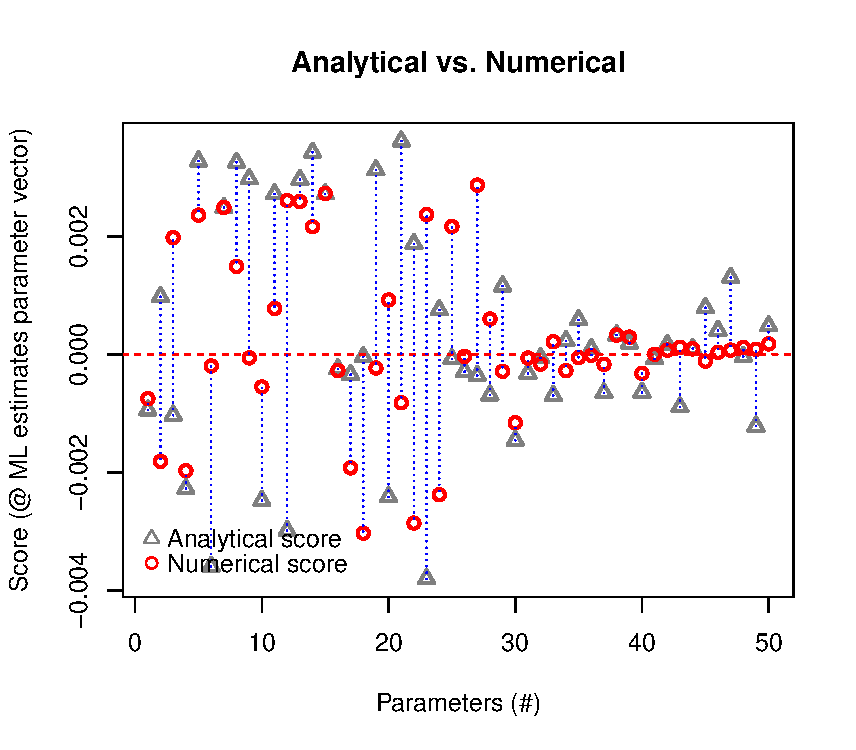
\includegraphics[scale = 0.5]{ScoreGausQTHT.pdf}
\caption{Ex.1: Quadratic FA + Heteroscedasticity.}
\label{fig:AppScoreSim1}
\end{subfigure}
~ %add desired spacing between images, e. g. ~, \quad, \qquad, \hfill etc. 
  %(or a blank line to force the subfigure onto a new line)
\begin{subfigure}[b]{0.45\textwidth}
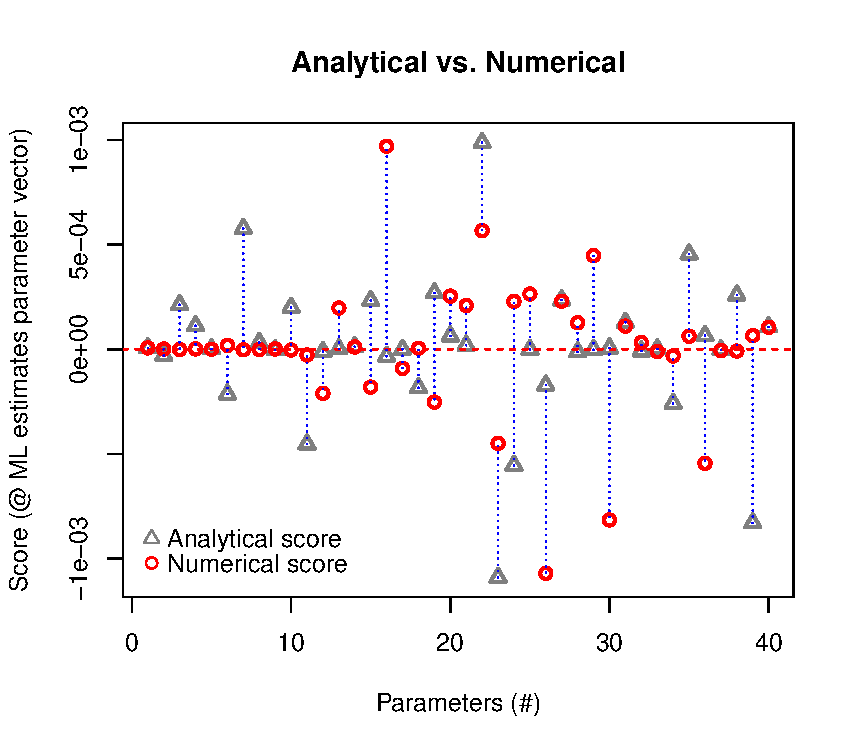
\includegraphics[scale = 0.5]{ScoreBinomInt.pdf}
\caption{Ex.2: IRT with interactions.}
\label{fig:AppScoreSim2}
\end{subfigure}
\\ 
\begin{subfigure}[b]{0.45\textwidth}
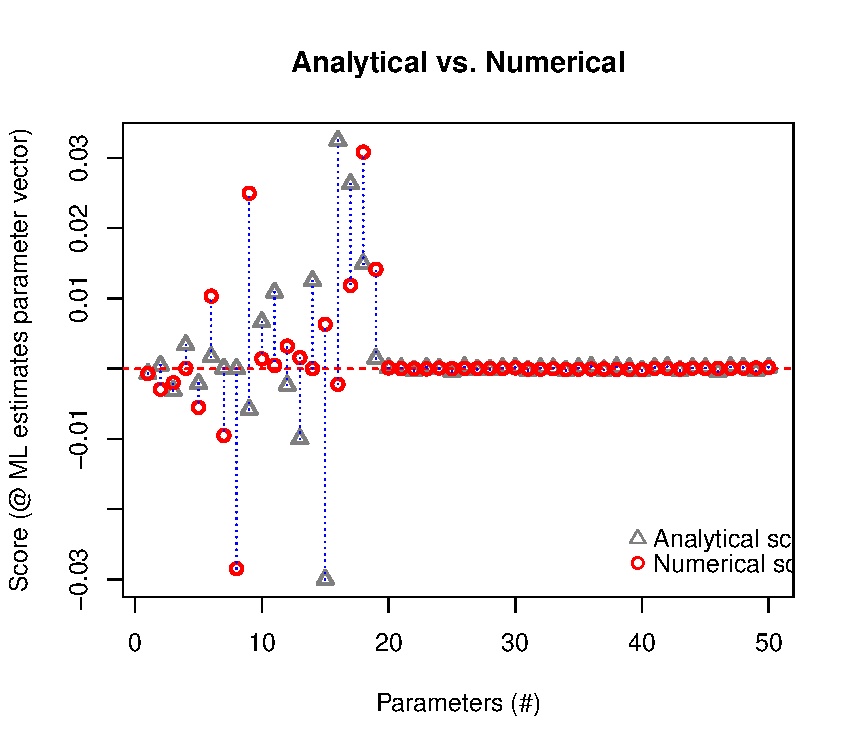
\includegraphics[scale = 0.5]{ScoreZIPlinQT.pdf}
\caption{Ex.3: ZI-Poisson LVM.}
\label{fig:AppScoreSim3}
\end{subfigure}
\caption{Score functions evaluated at $\hat{\Theta}$ for different models, $\mathbb{S}(\hat{\Theta})$.}
\label{fig:AppScore}
\end{figure}

\newpage

\subsection{Simulation results}

\begin{table}[h!]
%\begin{sidewaystable}[b!]
\centering \scriptsize{ %tiny %footnotesize
\rotatebox{90}{
\begin{tabular}{lccccccccccccccc}
& \multicolumn{15}{c}{\multirow{2}{*}{n = 100. Iterations to convergence: median: 39; mean: 46.1; min: 14; max: 338 (1,000/1,000 converged)}} \\ & \\
\cmidrule(lr){2-16}
& \multicolumn{3}{c}{$\alpha_{i0,\mu}$} & \multicolumn{3}{c}{$\alpha_{i1,\mu}$} & \multicolumn{3}{c}{$\alpha_{i2,\mu}$} & \multicolumn{3}{c}{$\alpha_{i0,\sigma}$} & \multicolumn{3}{c}{$\alpha_{i1,\sigma}$}\\ 
& RMSE & Bias & RB $(\%)$ & RMSE & Bias & RB $(\%)$ & RMSE & Bias & RB $(\%)$ & RMSE & Bias & RB $(\%)$ & RMSE & Bias & RB $(\%)$ \\ \cmidrule(lr){2-4} \cmidrule(lr){5-7} \cmidrule(lr){8-10} \cmidrule(lr){11-13} \cmidrule(lr){14-16}
Item 1 & 0.256 & 0.017 & -2.221 & 0.276 & 0.015 & 5.373 & 0.175 & -0.006 & -1.574 & 0.095 & -0.039 & -5.816 & 0.093 & -0.008 & 2.200 \\ 
Item 2 & 0.141 & -0.022 & -8.946 & 0.120 & 0.018 & -1.807 & 0.070 & -0.009 & -10.365 & 0.125 & -0.042 & 9.862 & 0.113 & -0.028 & 6.987 \\ 
Item 3 & 0.123 & -0.028 & -12.739 & 0.152 & -0.025 & 4.738 & 0.093 & 0.011 & -2.459 & 0.134 & -0.047 & 10.019 & 0.111 & -0.001 & 0.151 \\ 
Item 4 & 0.123 & 0.034 & 13.669 & 0.249 & 0.021 & 6.366 & 0.143 & -0.009 & -1.108 & 0.199 & 0.140 & -22.398 & 0.261 & 0.218 & -23.656 \\ 
Item 5 & 0.081 & -0.009 & -1.252 & 0.139 & -0.022 & -77.231 & 0.074 & 0.007 & -1.639 & 0.113 & -0.042 & 7.923 & 0.102 & -0.009 & 1.652 \\ 
\cmidrule(lr){2-16}

& \multicolumn{15}{c}{\multirow{2}{*}{n = 500. Iterations to convergence: median 56; mean: 66.2; min: 18; max: 419 (1,000/1,000 converged)}} \\ & \\
\cmidrule(lr){2-16}
& \multicolumn{3}{c}{$\alpha_{i0,\mu}$} & \multicolumn{3}{c}{$\alpha_{i1,\mu}$} & \multicolumn{3}{c}{$\alpha_{i2,\mu}$} & \multicolumn{3}{c}{$\alpha_{i0,\sigma}$} & \multicolumn{3}{c}{$\alpha_{i1,\sigma}$}\\ 
& RMSE & Bias & RB $(\%)$ & RMSE & Bias & RB $(\%)$ & RMSE & Bias & RB $(\%)$ & RMSE & Bias & RB $(\%)$ & RMSE & Bias & RB $(\%)$ \\ \cmidrule(lr){2-4} \cmidrule(lr){5-7} \cmidrule(lr){8-10} \cmidrule(lr){11-13} \cmidrule(lr){14-16}
Item 1 & 0.108 & 0.014 & -1.839 & 0.129 & 0.027 & 9.758 & 0.070 & -0.012 & -3.115 & 0.043 & -0.012 & -1.834 & 0.035 & 0.002 & -0.506 \\ 
Item 2 & 0.077 & -0.017 & -6.814 & 0.051 & 0.009 & -0.950 & 0.023 & -0.004 & -4.798 & 0.057 & -0.022 & 5.249 & 0.040 & -0.003 & 0.870 \\ 
Item 3 & 0.064 & -0.015 & -6.840 & 0.089 & -0.035 & 6.476 & 0.044 & 0.014 & -3.131 & 0.064 & -0.013 & 2.701 & 0.053 & 0.031 & -4.491 \\ 
Item 4 & 0.061 & 0.005 & 2.004 & 0.151 & 0.045 & 13.457 & 0.072 & -0.016 & -1.892 & 0.208 & 0.197 & -31.412 & 0.284 & 0.279 & -30.308 \\ 
Item 5 & 0.035 & -0.001 & -0.149 & 0.079 & -0.032 & -111.427 & 0.035 & 0.011 & -2.565 & 0.054 & -0.017 & 3.088 & 0.042 & 0.014 & -2.465 \\ 
\cmidrule(lr){2-16}
& \multicolumn{15}{c}{\multirow{2}{*}{n = 1,000. Iterations to convergence: median: 64; mean: 72.0; min: 20; max: 409 (1,000/1,000 converged)}} \\ & \\
\cmidrule(lr){2-16}
& \multicolumn{3}{c}{$\alpha_{i0,\mu}$} & \multicolumn{3}{c}{$\alpha_{i1,\mu}$} & \multicolumn{3}{c}{$\alpha_{i2,\mu}$} & \multicolumn{3}{c}{$\alpha_{i0,\sigma}$} & \multicolumn{3}{c}{$\alpha_{i1,\sigma}$}\\ 
& RMSE & Bias & RB $(\%)$ & RMSE & Bias & RB $(\%)$ & RMSE & Bias & RB $(\%)$ & RMSE & Bias & RB $(\%)$ & RMSE & Bias & RB $(\%)$ \\ \cmidrule(lr){2-4} \cmidrule(lr){5-7} \cmidrule(lr){8-10} \cmidrule(lr){11-13} \cmidrule(lr){14-16}
Item 1 & 0.078 & 0.015 & -1.877 & 0.102 & 0.042 & 15.109 & 0.051 & -0.018 & -4.713 & 0.035 & -0.015 & -2.167 & 0.026 & 0.008 & -2.148 \\ 
Item 2 & 0.069 & -0.025 & -10.325 & 0.042 & 0.022 & -2.192 & 0.019 & -0.008 & -9.189 & 0.046 & -0.023 & 5.324 & 0.029 & -0.001 & 0.199 \\ 
Item 3 & 0.057 & -0.022 & -10.217 & 0.089 & -0.051 & 9.463 & 0.042 & 0.025 & -5.686 & 0.048 & 0.010 & -2.095 & 0.080 & 0.073 & -10.736 \\ 
Item 4 & 0.054 & 0.012 & 4.728 & 0.147 & 0.075 & 22.711 & 0.068 & -0.036 & -4.280 & 0.254 & 0.249 & -39.737 & 0.353 & 0.351 & -38.161 \\ 
Item 5 & 0.027 & -0.006 & -0.821 & 0.080 & -0.048 & -166.841 & 0.034 & 0.020 & -4.920 & 0.042 & -0.010 & 1.865 & 0.044 & 0.033 & -5.908 \\ 
\cmidrule(lr){2-16}
\end{tabular}%
} % end rotate
} % end font size
\caption{Simulation Results: Quadratic Heteroscedastic Gaussian factor model, 5 items.}
\label{tab:A1Sim1a}
% \end{sidewaystable}
\end{table}

\clearpage

%%%%%

\hfill
\begin{table}[h!]
%\begin{sidewaystable}[b!]
\centering \tiny{ %tiny
\rotatebox{90}{
\begin{tabular}{lccccccccccccccc}
& \multicolumn{15}{c}{\multirow{2}{*}{n = 100. Iterations to convergence: median: 38; mean: 45.4; min: 17; max: 265 (1,000/1,000 converged)}} \\ & \\
\cmidrule(lr){2-16}
& \multicolumn{3}{c}{$\alpha_{i0,\mu}$} & \multicolumn{3}{c}{$\alpha_{i1,\mu}$} & \multicolumn{3}{c}{$\alpha_{i2,\mu}$} & \multicolumn{3}{c}{$\alpha_{i0,\sigma}$} & \multicolumn{3}{c}{$\alpha_{i1,\sigma}$}\\ 
& RMSE & Bias & RB $(\%)$ & RMSE & Bias & RB $(\%)$ & RMSE & Bias & RB $(\%)$ & RMSE & Bias & RB $(\%)$ & RMSE & Bias & RB $(\%)$ \\ \cmidrule(lr){2-4} \cmidrule(lr){5-7} \cmidrule(lr){8-10} \cmidrule(lr){11-13} \cmidrule(lr){14-16}
Item 1 & 0.123 & -0.002 & 0.295 & 0.118 & -0.005 & -1.383 & 0.077 & -0.001 & 0.177 & 0.081 & -0.027 & 30.727 & 0.085 & 0.006 & 5.270 \\ 
Item 2 & 0.082 & -0.005 & -2.175 & 0.095 & 0.002 & 2.009 & 0.058 & 0.003 & -0.779 & 0.091 & -0.036 & 7.684 & 0.100 & 0.009 & 2.960 \\ 
Item 3 & 0.102 & -0.002 & -0.731 & 0.133 & -0.005 & 1.247 & 0.076 & 0.007 & -1.037 & 0.101 & -0.030 & 7.634 & 0.108 & -0.001 & 0.242 \\ 
Item 4 & 0.161 & -0.005 & -2.169 & 0.177 & 0.000 & 0.050 & 0.107 & 0.007 & -0.712 & 0.107 & -0.036 & -244.523 & 0.111 & 0.014 & 5.593 \\ 
Item 5 & 0.084 & -0.003 & -0.362 & 0.105 & -0.000 & 0.106 & 0.062 & 0.005 & -0.814 & 0.105 & -0.026 & 4.010 & 0.112 & 0.005 & -1.396 \\ 
Item 6 & 0.223 & 0.003 & 1.034 & 0.195 & -0.001 & -0.208 & 0.138 & -0.004 & -0.701 & 0.079 & -0.027 & -5.180 & 0.086 & -0.000 & -6.293 \\ 
Item 7 & 0.074 & 0.003 & -0.292 & 0.080 & -0.001 & 0.158 & 0.047 & -0.002 & -3.635 & 0.091 & -0.034 & 5.745 & 0.089 & 0.014 & 3.846 \\ 
Item 8 & 0.094 & 0.001 & -0.143 & 0.126 & 0.000 & -0.012 & 0.070 & -0.002 & -0.232 & 0.104 & -0.034 & 7.142 & 0.117 & 0.007 & -21.822 \\ 
Item 9 & 0.314 & -0.010 & -3.061 & 0.424 & 0.011 & -1.735 & 0.227 & 0.000 & 0.024 & 0.089 & -0.026 & -2.623 & 0.089 & -0.006 & 1.137 \\ 
Item 10 & 0.209 & 0.009 & 31.837 & 0.319 & -0.000 & 0.002 & 0.161 & 0.002 & -0.216 & 0.091 & -0.029 & -4.757 & 0.090 & 0.008 & 1.570 \\  
\cmidrule(lr){2-16}

& \multicolumn{15}{c}{\multirow{2}{*}{n = 500. Iterations to convergence: median: 53; mean: 60.95; min: 15; max: 404 (1,000/1,000 converged)}} \\ & \\
\cmidrule(lr){2-16}
& \multicolumn{3}{c}{$\alpha_{i0,\mu}$} & \multicolumn{3}{c}{$\alpha_{i1,\mu}$} & \multicolumn{3}{c}{$\alpha_{i2,\mu}$} & \multicolumn{3}{c}{$\alpha_{i0,\sigma}$} & \multicolumn{3}{c}{$\alpha_{i1,\sigma}$}\\ 
& RMSE & Bias & RB $(\%)$ & RMSE & Bias & RB $(\%)$ & RMSE & Bias & RB $(\%)$ & RMSE & Bias & RB $(\%)$ & RMSE & Bias & RB $(\%)$ \\ \cmidrule(lr){2-4} \cmidrule(lr){5-7} \cmidrule(lr){8-10} \cmidrule(lr){11-13} \cmidrule(lr){14-16}
Item 1 & 0.056 & -0.003 & 0.434 & 0.056 & -0.003 & -0.731 & 0.034 & 0.002 & -0.499 & 0.035 & -0.005 & 5.813 & 0.036 & 0.000 & 0.136 \\ 
Item 2 & 0.035 & -0.003 & -1.323 & 0.053 & -0.004 & -4.432 & 0.028 & 0.001 & -0.341 & 0.036 & -0.003 & 0.614 & 0.038 & -0.003 & -1.142 \\ 
Item 3 & 0.048 & -0.006 & -2.581 & 0.082 & -0.006 & 1.460 & 0.040 & 0.004 & -0.530 & 0.044 & 0.013 & -3.404 & 0.053 & 0.031 & -8.179 \\ 
Item 4 & 0.074 & -0.005 & -2.100 & 0.112 & -0.009 & -1.058 & 0.056 & 0.003 & -0.274 & 0.040 & 0.002 & 16.358 & 0.042 & -0.011 & -4.479 \\ 
Item 5 & 0.040 & -0.005 & -0.676 & 0.067 & -0.005 & 1.134 & 0.032 & 0.002 & -0.403 & 0.045 & 0.014 & -2.136 & 0.054 & 0.032 & -9.443 \\ 
Item 6 & 0.097 & 0.006 & 1.976 & 0.100 & 0.004 & 0.629 & 0.064 & -0.002 & -0.385 & 0.033 & -0.007 & -1.389 & 0.036 & 0.001 & 20.186 \\ 
Item 7 & 0.035 & 0.001 & -0.093 & 0.035 & -0.000 & 0.048 & 0.018 & -0.001 & -1.604 & 0.038 & -0.005 & 0.804 & 0.037 & 0.002 & 0.482 \\ 
Item 8 & 0.043 & 0.004 & -0.788 & 0.088 & 0.006 & -1.327 & 0.043 & -0.002 & -0.190 & 0.040 & -0.000 & 0.090 & 0.044 & 0.002 & -5.280 \\ 
Item 9 & 0.134 & 0.002 & 0.524 & 0.194 & 0.000 & -0.029 & 0.087 & 0.001 & 0.202 & 0.043 & -0.007 & -0.712 & 0.038 & -0.002 & 0.344 \\ 
Item 10 & 0.102 & -0.008 & -28.089 & 0.149 & -0.003 & 0.638 & 0.071 & 0.005 & -0.522 & 0.042 & -0.001 & -0.190 & 0.038 & -0.001 & -0.280 \\ 
\cmidrule(lr){2-16}
& \multicolumn{15}{c}{\multirow{2}{*}{n = 1,000. Iterations to convergence: median: 64; mean: 75.1; min: 23; max: 482 (998/1,000 converged)}} \\ & \\
\cmidrule(lr){2-16}
& \multicolumn{3}{c}{$\alpha_{i0,\mu}$} & \multicolumn{3}{c}{$\alpha_{i1,\mu}$} & \multicolumn{3}{c}{$\alpha_{i2,\mu}$} & \multicolumn{3}{c}{$\alpha_{i0,\sigma}$} & \multicolumn{3}{c}{$\alpha_{i1,\sigma}$}\\ 
& RMSE & Bias & RB $(\%)$ & RMSE & Bias & RB $(\%)$ & RMSE & Bias & RB $(\%)$ & RMSE & Bias & RB $(\%)$ & RMSE & Bias & RB $(\%)$ \\ \cmidrule(lr){2-4} \cmidrule(lr){5-7} \cmidrule(lr){8-10} \cmidrule(lr){11-13} \cmidrule(lr){14-16}
Item 1 & 0.041 & -0.001 & 0.089 & 0.047 & -0.003 & -0.892 & 0.027 & 0.002 & -0.647 & 0.024 & -0.003 & 3.039 & 0.025 & -0.001 & -1.284 \\ 
Item 2 & 0.025 & -0.001 & -0.582 & 0.046 & -0.003 & -3.284 & 0.022 & 0.002 & -0.564 & 0.027 & 0.000 & -0.014 & 0.027 & -0.004 & -1.314 \\ 
Item 3 & 0.037 & -0.009 & -4.103 & 0.075 & -0.007 & 1.612 & 0.035 & 0.006 & -0.945 & 0.037 & 0.019 & -4.811 & 0.049 & 0.040 & -10.499 \\ 
Item 4 & 0.056 & -0.004 & -1.601 & 0.098 & -0.010 & -1.210 & 0.046 & 0.006 & -0.615 & 0.030 & 0.007 & 50.153 & 0.032 & -0.015 & -6.079 \\ 
Item 5 & 0.031 & -0.006 & -0.806 & 0.060 & -0.005 & 1.135 & 0.028 & 0.005 & -0.866 & 0.037 & 0.021 & -3.274 & 0.048 & 0.038 & -11.237 \\ 
Item 6 & 0.069 & 0.004 & 1.595 & 0.081 & 0.007 & 0.991 & 0.048 & -0.001 & -0.098 & 0.023 & -0.001 & -0.258 & 0.024 & 0.000 & 5.483 \\ 
Item 7 & 0.027 & -0.001 & 0.052 & 0.026 & 0.000 & -0.055 & 0.013 & -0.001 & -2.428 & 0.029 & -0.001 & 0.209 & 0.026 & 0.001 & 0.176 \\ 
Item 8 & 0.033 & 0.003 & -0.604 & 0.082 & 0.009 & -1.842 & 0.037 & -0.004 & -0.510 & 0.029 & 0.002 & -0.320 & 0.029 & -0.000 & 1.081 \\ 
Item 9 & 0.096 & -0.001 & -0.311 & 0.136 & 0.015 & -2.379 & 0.059 & -0.007 & -1.092 & 0.033 & -0.003 & -0.338 & 0.027 & 0.000 & -0.054 \\ 
Item 10 & 0.072 & -0.005 & -17.198 & 0.127 & -0.009 & 1.619 & 0.055 & 0.003 & -0.294 & 0.032 & 0.003 & 0.500 & 0.029 & -0.007 & -1.229 \\ 
\cmidrule(lr){2-16}
\end{tabular}%
} % end rotate
} % end font size
\caption{Simulation Results: Quadratic Heteroscedastic Gaussian factor model, 10 items.}
\label{tab:A1Sim1b}
% \end{sidewaystable}
\end{table}

\clearpage
% \restoregeometry

\hfill
\begin{table}[h!]
%\begin{sidewaystable}[b!]
\centering \footnotesize{ %tiny
\rotatebox{90}{
\begin{tabular}{lcccccccccccc}
& \multicolumn{12}{c}{\multirow{2}{*}{n = 1,000. Iterations to convergence: median: 214; mean: 257.4; min: 83; max: 699 (807/1,000 converged)}} \\ & \\
\cmidrule(lr){2-13}
& \multicolumn{3}{c}{$\alpha_{i0,\pi}$} & \multicolumn{3}{c}{$\alpha_{i1,\pi}$} & \multicolumn{3}{c}{$\alpha_{i2,\pi}$} & \multicolumn{3}{c}{$\alpha_{i3,\pi}$} \\ 
& RMSE & Bias & RB $(\%)$ & RMSE & Bias & RB $(\%)$ & RMSE & Bias & RB $(\%)$ & RMSE & Bias & RB $(\%)$ \\ \cmidrule(lr){2-4} \cmidrule(lr){5-7} \cmidrule(lr){8-10} \cmidrule(lr){11-13}
Item 1 & 0.154 & -0.040 & 2.365 & 0.182 & -0.033 & 7.288 & 0.217 & -0.017 & 2.337 & 0.229 & -0.054 & 6.024 \\ 
Item 2 & 0.182 & -0.046 & 12.175 & 0.399 & 0.151 & 7.855 & 0.352 & -0.004 & -0.691 & 0.469 & -0.034 & 18.477 \\ 
Item 3 & 0.091 & -0.016 & 4.158 & 0.166 & 0.003 & 1.110 & 0.213 & -0.009 & -1.981 & 0.353 & 0.064 & 4.303 \\ 
Item 4 & 0.100 & 0.023 & 2.613 & 0.115 & -0.023 & 5.774 & 0.191 & -0.035 & 6.162 & 0.168 & 0.011 & 13.180 \\ 
Item 5 & 0.098 & -0.010 & -8.580 & 0.193 & 0.045 & 3.418 & 0.211 & -0.012 & -1.799 & 0.236 & 0.008 & 2.554 \\ 
Item 6 & 4.521 & -0.425 & 23.433 & 4.641 & 0.393 & 24.084 & 7.195 & -0.553 & 31.474 & 7.305 & -0.655 & 42.943 \\ 
Item 7 & 0.079 & 0.017 & 1.516 & 0.102 & -0.004 & 4.460 & 0.131 & 0.005 & 3.283 & 0.130 & 0.006 & 4.573 \\ 
Item 8 & 0.151 & -0.039 & 2.562 & 0.236 & 0.040 & 2.985 & 0.223 & -0.033 & -10.515 & 0.263 & 0.012 & 1.197 \\ 
Item 9 & 0.165 & 0.046 & 2.590 & 0.223 & 0.038 & 9.024 & 0.258 & -0.031 & 15.398 & 0.313 & -0.061 & 4.411 \\ 
Item 10 & 0.219 & 0.077 & 8.202 & 0.383 & -0.119 & 8.222 & 0.318 & 0.115 & 33.903 & 0.431 & -0.129 & 11.875 \\
\cmidrule(lr){2-13}
\end{tabular}%
} % end rotate
} % end font size
\caption{Simulation Results: Interaction IRT model, 10 items.}
\label{tab:A1Sim2}
% \end{sidewaystable}
\end{table}

\clearpage

\begin{table}[h!]
%\begin{sidewaystable}[b!]
\centering \footnotesize{ %tiny %footnotesize
\rotatebox{90}{
\begin{tabular}{lccccccccccccccc}
\cmidrule(lr){2-16}
& \multicolumn{15}{c}{\multirow{2}{*}{n = 500. Iterations to convergence: median: 124; mean: 146.5; min: 20; max: 694 (999/1,000 converged)}} \\ & \\
\cmidrule(lr){2-16}
& \multicolumn{3}{c}{$\alpha_{i0,\lambda}$} & \multicolumn{3}{c}{$\alpha_{i1,\lambda}$} & \multicolumn{3}{c}{$\alpha_{i0,\pi}$} & \multicolumn{3}{c}{$\alpha_{i1,\pi}$} & \multicolumn{3}{c}{$\alpha_{i2,\pi}$}\\ 
& RMSE & Bias & RB $(\%)$ & RMSE & Bias & RB $(\%)$ & RMSE & Bias & RB $(\%)$ & RMSE & Bias & RB $(\%)$ & RMSE & Bias & RB $(\%)$ \\ \cmidrule(lr){2-4} \cmidrule(lr){5-7} \cmidrule(lr){8-10} \cmidrule(lr){11-13} \cmidrule(lr){14-16}
Item 1 & 0.022 & -0.002 & -0.120 & 0.020 & 0.000 & -0.290 & 0.135 & 0.007 & 125.120 & 0.175 & -0.025 & 20.326 & 0.156 & -0.010 & 1.297 \\ 
  Item 2 & 0.041 & -0.007 & -0.378 & 0.023 & 0.005 & -1.069 & 0.151 & -0.005 & -0.524 & 0.246 & -0.042 & 7.781 & 0.213 & 0.002 & -0.159 \\ 
  Item 3 & 0.040 & -0.008 & -0.565 & 0.028 & 0.003 & -0.883 & 0.142 & -0.012 & 3.530 & 0.202 & -0.028 & 3.339 & 0.149 & -0.012 & 2.156 \\ 
  Item 4 & 0.034 & -0.002 & -0.188 & 0.029 & 0.001 & 8.403 & 0.157 & 0.015 & -41.309 & 0.295 & -0.031 & -4.403 & 0.307 & -0.037 & 2.679 \\ 
  Item 5 & 0.048 & -0.010 & -0.631 & 0.027 & 0.006 & -0.957 & 0.153 & -0.012 & 4.183 & 0.304 & -0.048 & 9.060 & 0.300 & -0.017 & 1.307 \\ 
  Item 6 & 0.036 & 0.009 & 0.260 & 0.018 & -0.006 & -1.235 & 0.133 & 0.015 & 6.015 & 0.173 & -0.012 & -1.266 & 0.118 & 0.004 & -0.642 \\ 
  Item 7 & 0.044 & -0.009 & -0.363 & 0.024 & 0.007 & -1.093 & 0.128 & -0.001 & -0.146 & 0.131 & -0.013 & -6.173 & 0.109 & 0.001 & -0.157 \\ 
  Item 8 & 0.033 & -0.008 & -0.220 & 0.017 & 0.005 & -0.994 & 0.148 & 0.015 & 11.536 & 0.252 & -0.044 & -4.399 & 0.204 & 0.002 & -0.137 \\ 
  Item 9 & 0.071 & 0.018 & 0.524 & 0.032 & -0.012 & -1.252 & 0.148 & 0.006 & 0.645 & 0.230 & -0.051 & 20.311 & 0.201 & -0.001 & 0.052 \\ 
  Item 10 & 0.058 & 0.010 & 0.893 & 0.036 & -0.008 & -1.302 & 0.133 & 0.005 & 3.540 & 0.197 & -0.018 & -16.627 & 0.172 & -0.004 & 0.624 \\ 
\cmidrule(lr){2-16}
& \multicolumn{15}{c}{\multirow{2}{*}{n = 1,000. Iterations to convergence: median: 148; mean: 172.6; min: 31; max: 697 (991/1,000 converged)}} \\ & \\
\cmidrule(lr){2-16}
& \multicolumn{3}{c}{$\alpha_{i0,\lambda}$} & \multicolumn{3}{c}{$\alpha_{i1,\lambda}$} & \multicolumn{3}{c}{$\alpha_{i0,\pi}$} & \multicolumn{3}{c}{$\alpha_{i1,\pi}$} & \multicolumn{3}{c}{$\alpha_{i2,\pi}$}\\ 
& RMSE & Bias & RB $(\%)$ & RMSE & Bias & RB $(\%)$ & RMSE & Bias & RB $(\%)$ & RMSE & Bias & RB $(\%)$ & RMSE & Bias & RB $(\%)$ \\ \cmidrule(lr){2-4} \cmidrule(lr){5-7} \cmidrule(lr){8-10} \cmidrule(lr){11-13} \cmidrule(lr){14-16}
Item 1 & 0.016 & -0.002 & -0.107 & 0.013 & 0.001 & -1.278 & 0.090 & -0.004 & -73.439 & 0.131 & -0.031 & 25.825 & 0.107 & 0.014 & -1.748 \\ 
Item 2 & 0.031 & -0.009 & -0.480 & 0.019 & 0.007 & -1.447 & 0.107 & -0.012 & -1.238 & 0.183 & -0.052 & 9.630 & 0.153 & 0.027 & -1.929 \\ 
Item 3 & 0.029 & -0.008 & -0.521 & 0.020 & 0.005 & -1.281 & 0.104 & -0.019 & 5.547 & 0.157 & -0.033 & 3.993 & 0.111 & -0.004 & 0.772 \\ 
Item 4 & 0.024 & -0.000 & -0.033 & 0.020 & -0.000 & -1.249 & 0.113 & 0.019 & -51.685 & 0.222 & -0.061 & -8.769 & 0.217 & 0.002 & -0.121 \\ 
Item 5 & 0.038 & -0.012 & -0.746 & 0.023 & 0.008 & -1.272 & 0.106 & -0.012 & 4.160 & 0.221 & -0.058 & 11.012 & 0.221 & 0.008 & -0.649 \\ 
Item 6 & 0.030 & 0.011 & 0.321 & 0.017 & -0.007 & -1.433 & 0.099 & 0.018 & 7.083 & 0.123 & -0.026 & -2.682 & 0.084 & 0.013 & -2.139 \\ 
Item 7 & 0.035 & -0.012 & -0.471 & 0.021 & 0.008 & -1.285 & 0.085 & 0.002 & 0.373 & 0.098 & -0.018 & -8.766 & 0.076 & 0.008 & -1.473 \\ 
Item 8 & 0.027 & -0.010 & -0.261 & 0.015 & 0.006 & -1.281 & 0.111 & 0.016 & 12.503 & 0.197 & -0.045 & -4.469 & 0.148 & 0.012 & -1.007 \\ 
Item 9 & 0.059 & 0.023 & 0.662 & 0.031 & -0.016 & -1.616 & 0.102 & -0.006 & -0.656 & 0.172 & -0.049 & 19.556 & 0.146 & 0.027 & -1.935 \\ 
Item 10 & 0.044 & 0.012 & 1.061 & 0.027 & -0.009 & -1.501 & 0.095 & 0.004 & 2.287 & 0.141 & -0.019 & -17.539 & 0.121 & 0.004 & -0.546 \\ 
\cmidrule(lr){2-16}
\end{tabular}%
} % end rotate
} % end font size
\caption{Simulation Results: ZIP-LVM with quadratic `pure zero' state probability, 10 items.}
\label{tab:A1Sim3}
% \end{sidewaystable}
\end{table}

\clearpage

\bibliographystyle{apalike}
\bibliography{Bibliography}

\end{document}
